\chapter{井筒清洁工具性能评价与作业参数优选研究}
\label{chap:r46-5}

本项研究围绕四合一通刮刷磁集成式工具、大容量强磁吸附工具、多功能过滤工具、可变径刮管工具和三合一脉冲式冲刮刷工具，形成室内测试评价工艺。已开展冲砂、铁屑运移、菱形刮板、斜齿形刮板、套磨铣、毛刷刷洗和磁铁吸附七项实验，获得清洁部件功能及套磨铣作业性能的评价结果。

作业参数优选采用第四章的四组套磨铣实验数据，按工具和工件材料分别建立性能预测模型，以钻速为效率指标，同时考虑工作扭矩和磨损量。通过六种算法比较、五折交叉验证、候选工况搜索及Pareto非支配筛选，形成钻压与转速的智能优化方法。

\section{研发清洁工具的实验评价方法}
\label{sec:r46-5.1}
\label{guaban}

% 姚老师待修订范围：5.1及5.1.1—5.1.4；提示仅保留于源码注释和PR说明。

评价工艺包含30项方法：共性检查4项、四合一工具5项、强磁吸附工具6项、过滤工具5项、可变径工具4项、三合一工具6项。各方法明确试验对象、可控工况、测量指标和试前试后检查。表5-1列出方法组成及对应的评价要求；具体实施结果按本章刮板、毛刷、磁吸及套磨铣试验分别报告。

\begin{table}[H]
\centering
\setstretch{1}
\fontsize{12}{15}\selectfont
\setlength{\tabcolsep}{3pt}
\renewcommand{\arraystretch}{1.5}
\caption{五类研发工具的实验评价重点}\label{tab:r46-5-1}
\begin{tabular}{>{\centering\arraybackslash}m{0.219162\dimexpr\linewidth-6\tabcolsep-4\arrayrulewidth\relax}>{\centering\arraybackslash}m{0.445210\dimexpr\linewidth-6\tabcolsep-4\arrayrulewidth\relax}>{\centering\arraybackslash}m{0.335629\dimexpr\linewidth-6\tabcolsep-4\arrayrulewidth\relax}}
\toprule
 方法分组 & 方法组成 & 主要评价内容 \\ \midrule
共性检查 4项 & 尺寸与接口检查；通径与循环检查；拉扭承载评价；循环磨损与功能复验 & 设计尺寸、泄漏及流通状态、载荷响应、试后尺寸与功能保持 \\ 
四合一工具 5项 & 通过性；周向刮刷覆盖；刮板除垢；毛刷刷洗；磁吸与模块配合 & 通、刮、刷、磁功能，360°覆盖、阻力、去除量和模块状态 \\ 
大容量强磁 6项 & 静态拉脱；磁场分布；动态捕集；有效容量；带屑保持；耐温后复测 & 吸附力、捕集量、容量及热前热后性能；对应本型号合同指标 \\ 
多功能过滤 5项 & 通径；分级截留；存储容量；旋转与压差；启闭及清理复测 & 流通能力、截留率、碎屑储量和清理后功能 \\ 
可变径刮管 4项 & 小径通过；投球张开；两种套管刮管；复位及循环动作 & 9-5/8″与7″套管适应性、张开/收拢尺寸、动作保持及卡滞 \\ 
三合一工具 6项 & 脉冲波形；喷头旋转；液压刮管动作；密封筒通过及筛盲管清洁；冲刮刷协同；防卡与热态复验 & 4.75″密封筒通过、5-1/2″筛盲管清洁，脉冲、覆盖、负载和耐温功能 \\ \bottomrule
\end{tabular}
\end{table}

\subsection{刮板刮削效果评价}
\label{sec:r46-5.1.1}

采用转盘式台架，以重晶石粉与硫铝酸盐水泥按质量比3\ensuremath{\mathbin{:}}4制成的模拟硬垢为对象。垢样随转盘运动，刮板由弹簧提供压紧作用；限位机构约束五个自由度，保留压紧方向的浮动。试验平均线速度约0.05 m/s，单次刮削行程约0.5 m，用于比较菱形及斜齿形刮板的去除量和排屑状态。

\begin{figure}[H]
\centering
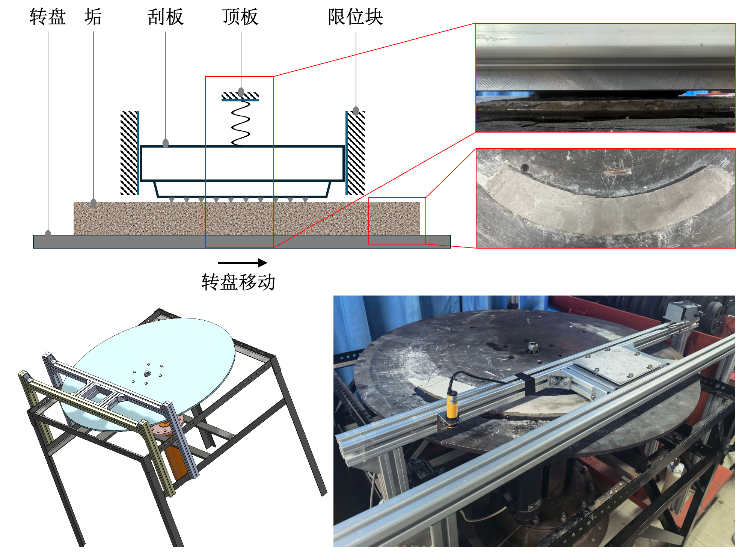
\includegraphics[width=123.000mm,height=0.76\textheight,keepaspectratio]{figure/research4-6/fig5-01-1.png}
\caption{刮板除垢评价装置及装夹方式}
\label{fig:r46-5-1}
\end{figure}

分别测量弹簧原长、参考预紧状态及刮削后的特征尺寸，结合横梁挠曲和沟槽累积坑深回算弹簧压缩估计值δs。单次刮削厚度δc为同一测点相邻两次累积坑深的增量。照片中的预设参考压缩量与关系图中的回算量分别记录，测量原理见图5-2。

\begin{figure}[H]
\centering
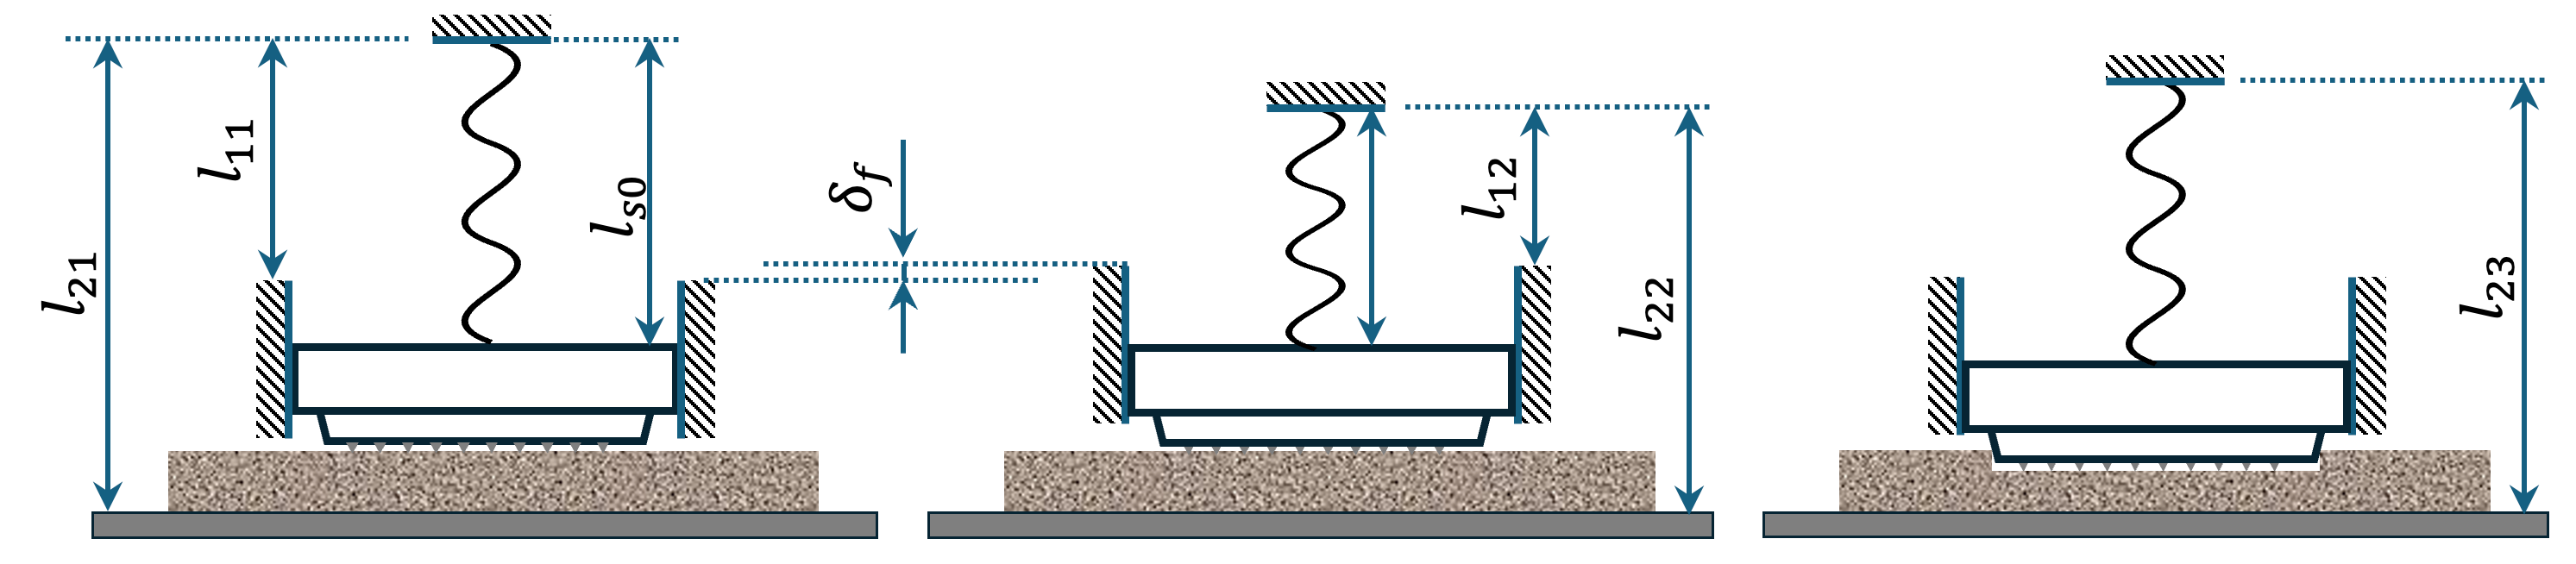
\includegraphics[width=145.000mm,height=0.76\textheight,keepaspectratio]{figure/research4-6/fig5-02-1.png}
\caption{弹簧压缩量与刮削厚度的测量原理}
\label{fig:r46-5-2}
\end{figure}

菱形刮板的逐次刮削记录中，δs约为3.9、5.5和7.1 mm时，单次厚度分别约为0.85、0.71和0.64 mm；约7.3 mm时降至0.11 mm，约9.6 mm时为0.08 mm（图5-3）。约7.2 mm附近出现明显转折。该组结果说明，预紧量应与刀齿接触、浮动行程和容屑空间共同匹配。

\begin{figure}[H]
\centering
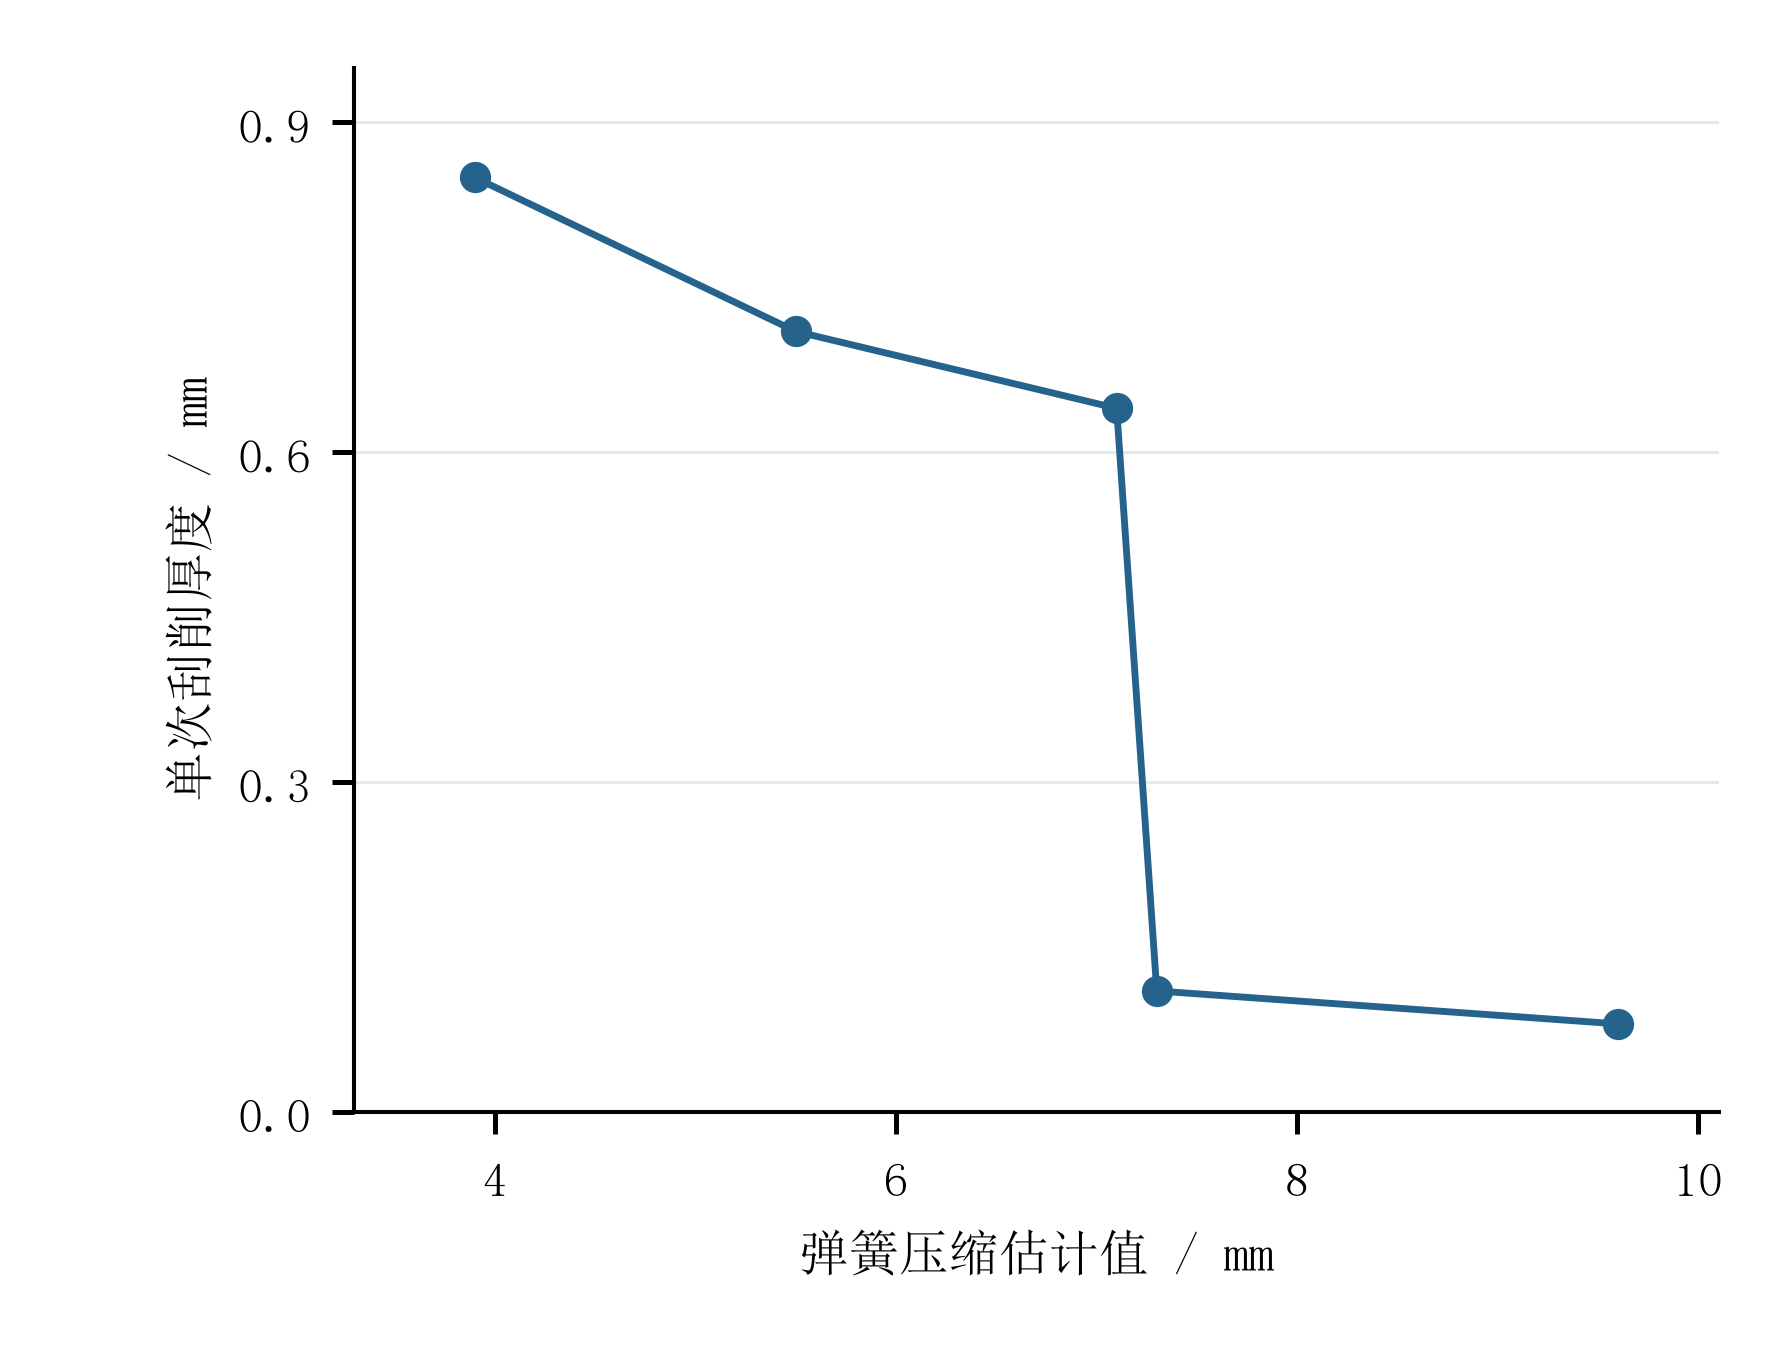
\includegraphics[width=142.000mm,height=0.76\textheight,keepaspectratio]{figure/research4-6/fig5-03-1.png}
\caption{菱形刮板单次刮削厚度与弹簧压缩估计值}
\label{fig:r46-5-3}
\end{figure}

斜齿形刮板的五组回算压缩量为7.21、9.68、10.11、10.83和11.26 mm，单次刮削厚度依次为0.235、0.150、0.295、0.050和0.150 mm，最大记录值对应10.11 mm工况（图5-4）。累积坑深由0.235 mm增至0.880 mm，单次增量呈非单调变化，选参需结合逐次沟槽加深和齿面排屑状态。

\begin{figure}[H]
\centering
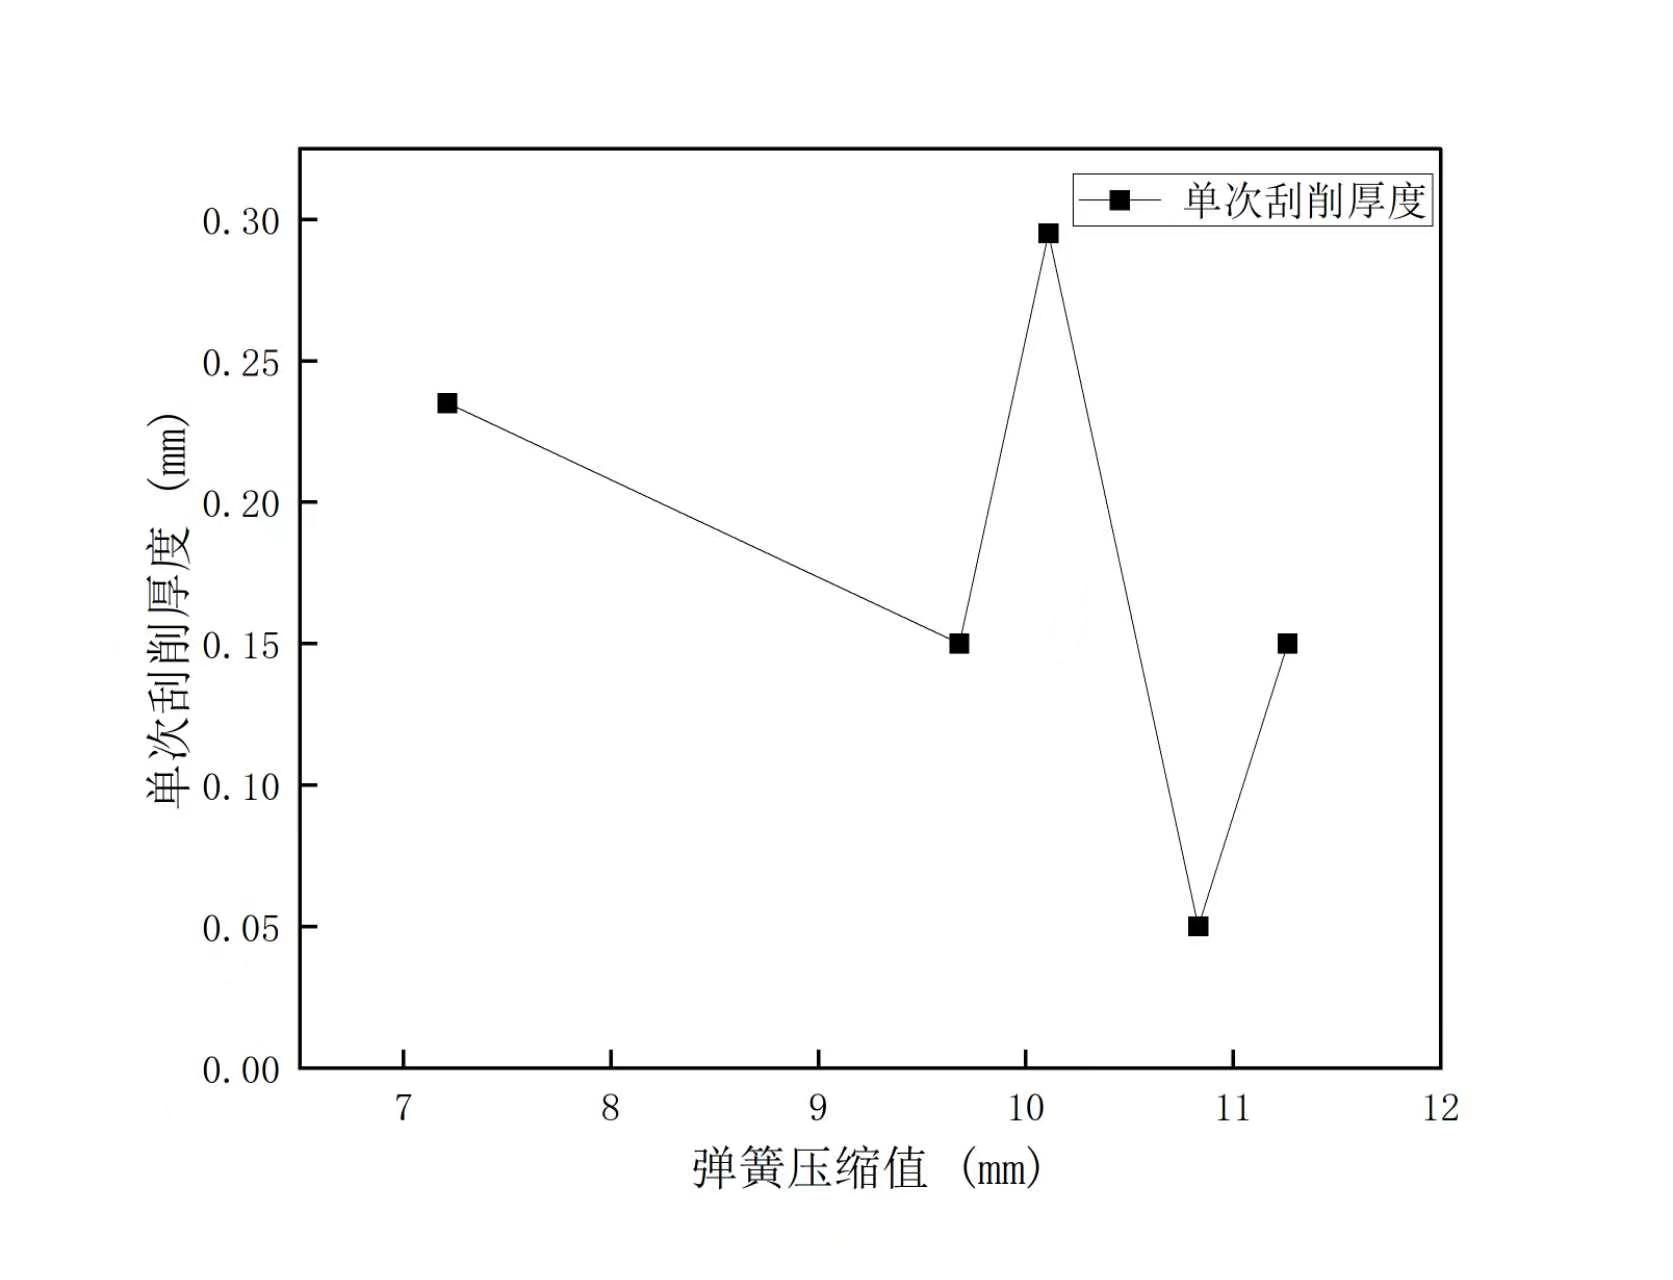
\includegraphics[width=142.000mm,height=0.76\textheight,keepaspectratio]{figure/research4-6/fig5-04-1.jpg}
\caption{斜齿形刮板单次刮削厚度与弹簧压缩量}
\label{fig:r46-5-4}
\end{figure}

两种刮板均在模拟硬垢上形成连续沟槽，切屑包含细粉和脆性崩碎块。试后齿面可见附着层及容屑槽充填；斜向刀齿和中部梯形齿的接触、容屑形式不同。刮板选用以单位行程去除量和齿槽状态共同评价，循环排屑用于维持后续刮削能力。

\begin{figure}[H]
\centering
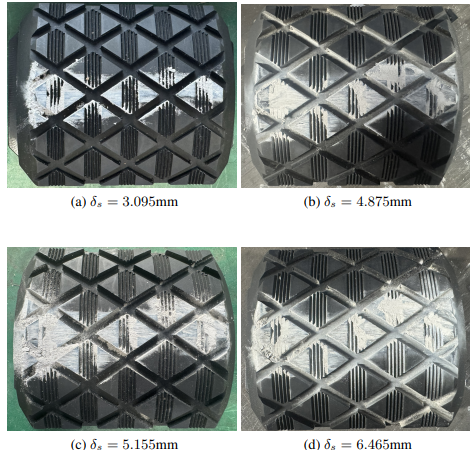
\includegraphics[width=142.000mm,height=0.76\textheight,keepaspectratio]{figure/research4-6/fig5-05-1.png}
\caption{刮削后刀齿表面形貌及容屑情况}
\label{fig:r46-5-5}
\end{figure}

\subsection{毛刷刷洗效果评价}
\label{sec:r46-5.1.2}

毛刷试验沿用转盘台架，以同一刷块分别对模拟硬垢和蜡垢刷洗一次，记录预紧状态、测点位置变化及刷体形貌。硬垢组弹簧压缩量为6.13 mm，蜡垢组按记录取14.06 mm；弹簧刚度约22.5 N/mm，对应估算压紧力约138 N和316 N。两组结果分别与各自预紧条件对应。

以顶板顶部测量基面至垢面的距离L₂为位置量，取四个测点的均值，按“刷洗后值减去预紧后值”计算ΔL₂。硬垢组为+0.465 mm，蜡垢组为−0.790 mm（表5-2）。蜡垢的负变化对应测点处垢面升高，结合照片中的推挤、涂抹和刷丝黏附分析其形貌变化。

\begin{table}[H]
\centering
\setstretch{1}
\fontsize{12}{15}\selectfont
\setlength{\tabcolsep}{3pt}
\renewcommand{\arraystretch}{1.5}
\caption{毛刷刷洗工况及测点位置变化}\label{tab:r46-5-2}
\begin{tabular}{>{\centering\arraybackslash}m{0.184948\dimexpr\linewidth-12\tabcolsep-7\arrayrulewidth\relax}>{\centering\arraybackslash}m{0.143875\dimexpr\linewidth-12\tabcolsep-7\arrayrulewidth\relax}>{\centering\arraybackslash}m{0.150640\dimexpr\linewidth-12\tabcolsep-7\arrayrulewidth\relax}>{\centering\arraybackslash}m{0.178062\dimexpr\linewidth-12\tabcolsep-7\arrayrulewidth\relax}>{\centering\arraybackslash}m{0.178062\dimexpr\linewidth-12\tabcolsep-7\arrayrulewidth\relax}>{\centering\arraybackslash}m{0.164412\dimexpr\linewidth-12\tabcolsep-7\arrayrulewidth\relax}}
\toprule
 垢样 & 弹簧压缩量\newline{}(mm) & 估算压紧力\newline{}(N) & 预紧后L₂\newline{}(mm) & 刷洗后L₂\newline{}(mm) & ΔL₂\newline{}(mm) \\ \midrule
模拟硬垢 & 6.13 & 138 & 89.510 & 89.975 & +0.465 \\ 
模拟蜡垢 & 14.06 & 316 & 79.920 & 79.130 & −0.790 \\ \bottomrule
\end{tabular}
\end{table}

硬垢刷洗后以表面划擦为主，刷体残留少量粉状垢屑；蜡垢出现涂抹及局部基体露出，刷丝黏附大量蜡质（图5-6）。刮板用于硬垢主体去除，毛刷用于细屑和蜡质附着物的清理，两者配合循环排屑形成机械清洁工艺。刷体固定、保养及维修检查参考T/GRM 112—2025相应条款。

\begin{figure}[H]
\centering
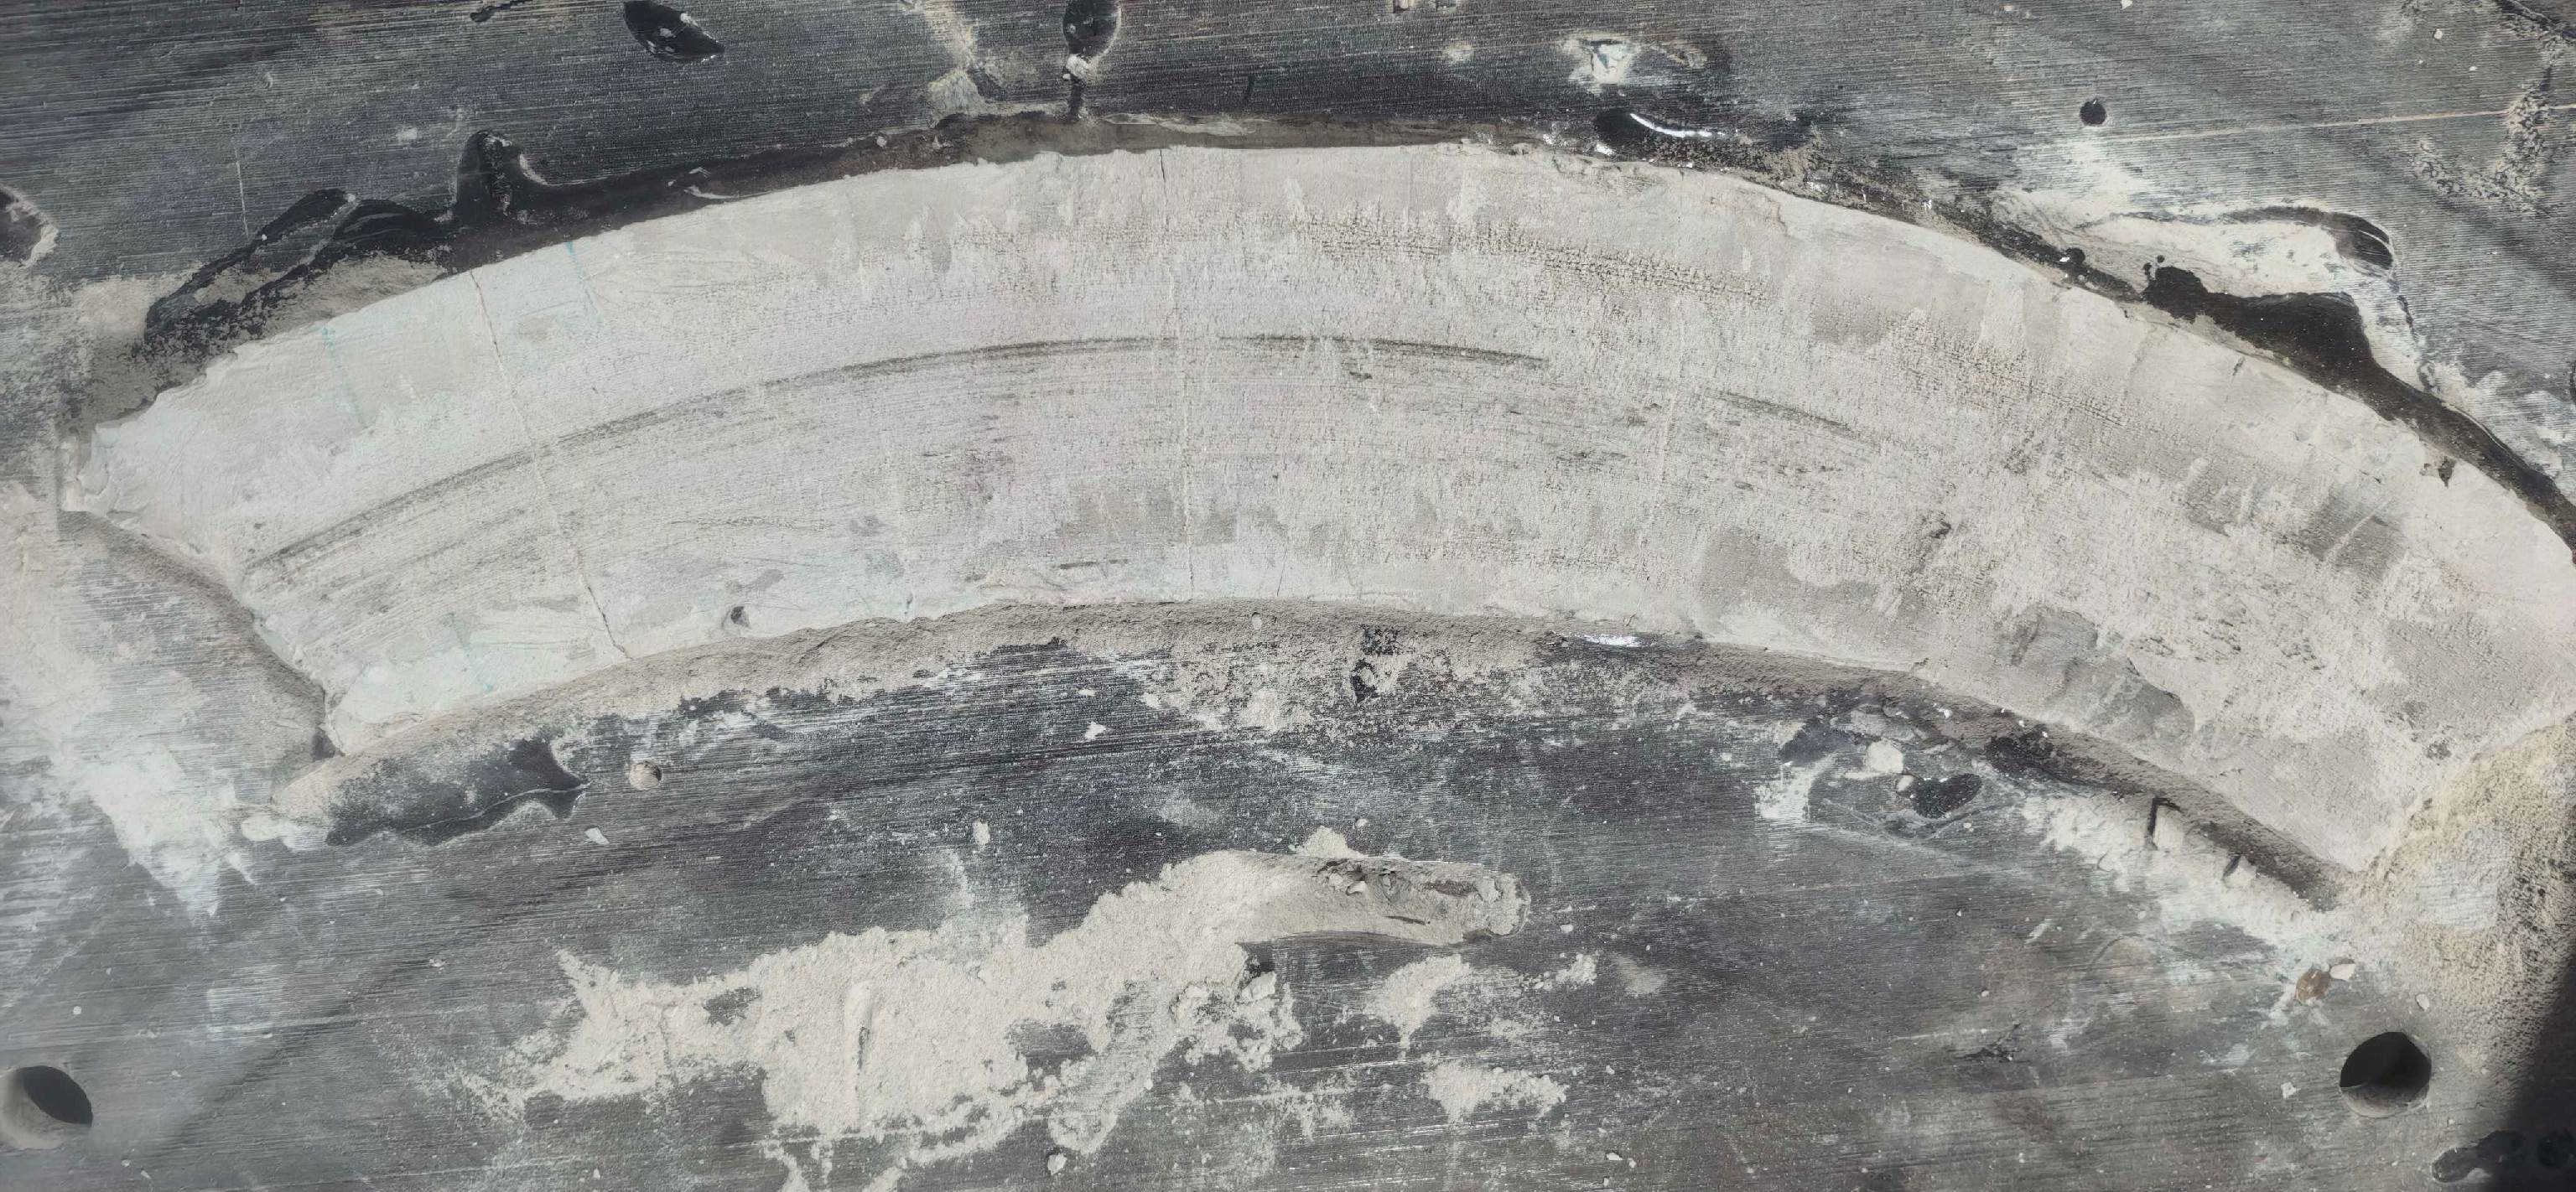
\includegraphics[width=70.000mm,height=0.76\textheight,keepaspectratio]{figure/research4-6/fig5-06-1.jpg}
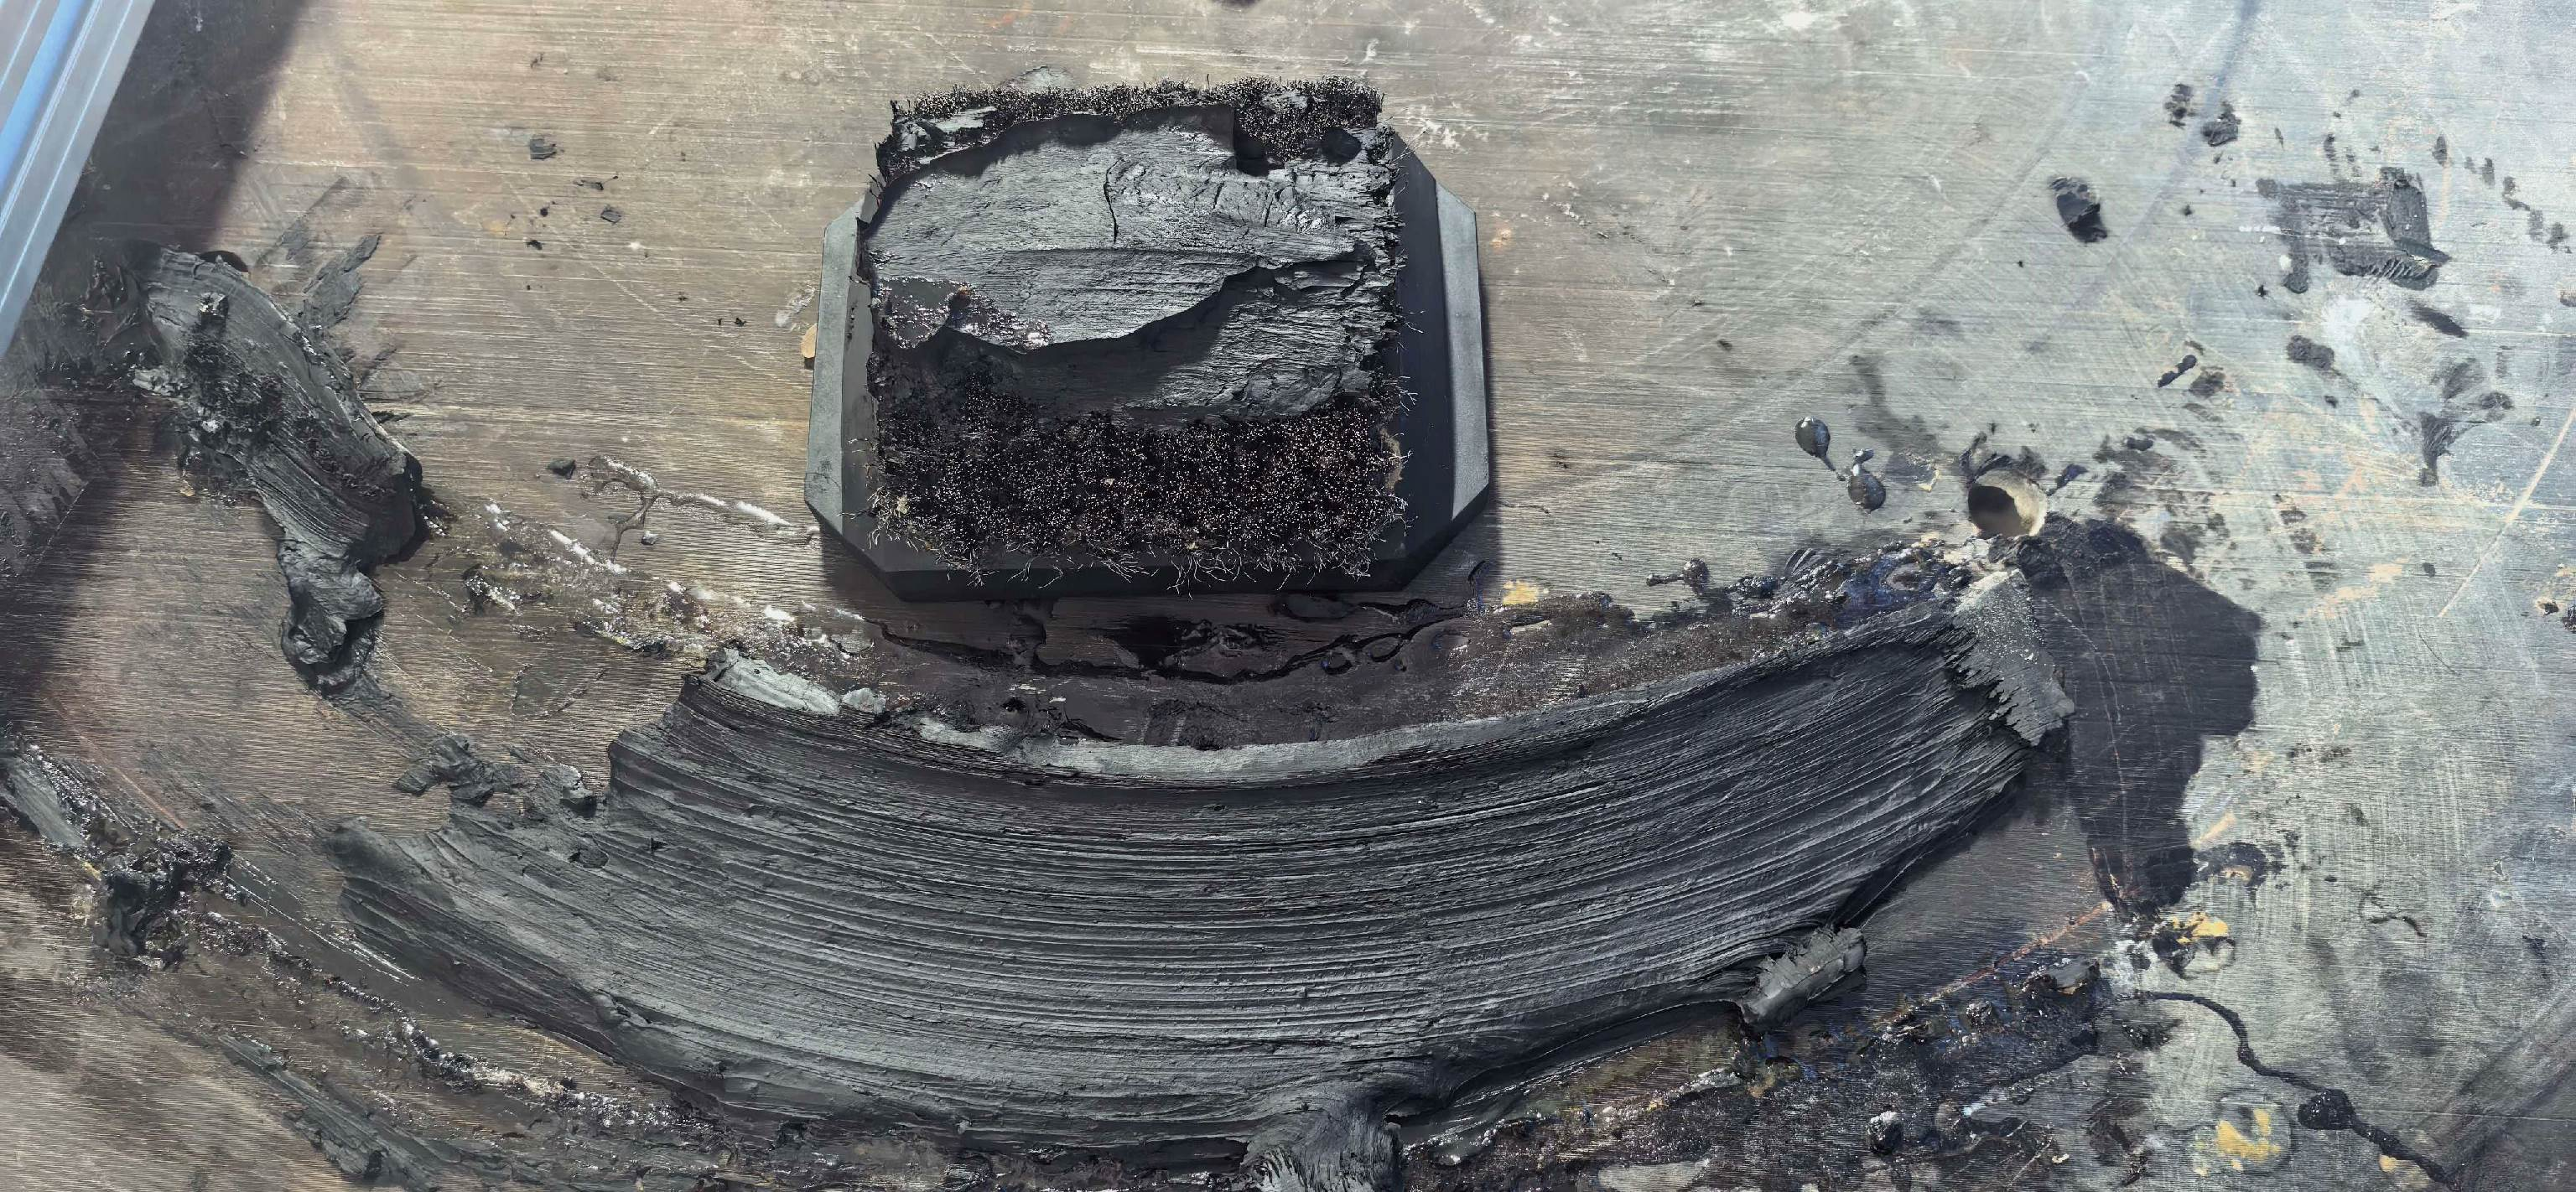
\includegraphics[width=70.000mm,height=0.76\textheight,keepaspectratio]{figure/research4-6/fig5-06-2.jpg}
\caption{硬垢与蜡垢刷洗后的垢面及刷体形貌}
\label{fig:r46-5-6}
\end{figure}

\subsection{四合一强磁模块吸附力评价}
\label{sec:r46-5.1.3}

采用由磁铁、45号钢圆柱试件、拉力传感器和千分头组成的轴向拉脱装置，见图5-7。试件直径1.8 cm，端面接触面积约2.545 cm²；在同一贴合位置缓慢牵引，记录脱离瞬间的拉力峰值，重复测定8次。试样为四合一工具的烧结钐钴强磁模块。

\begin{figure}[H]
\centering
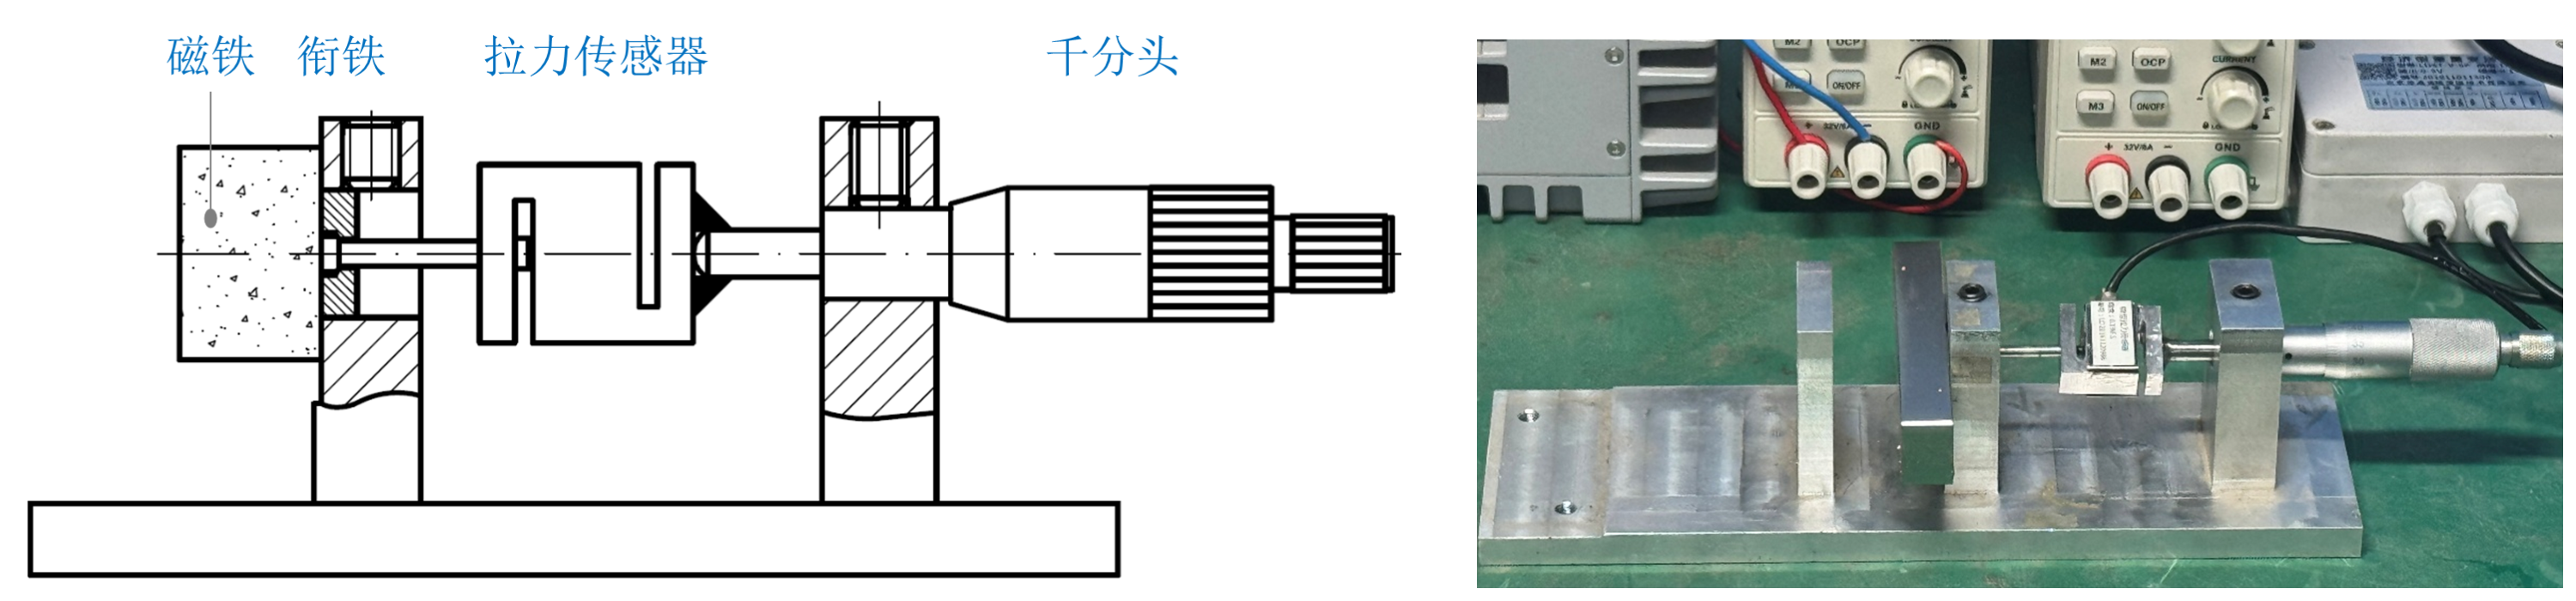
\includegraphics[width=145.000mm,height=0.76\textheight,keepaspectratio]{figure/research4-6/fig5-07-1.png}
\caption{磁铁吸附力测试装置原理与实物}
\label{fig:r46-5-7}
\end{figure}

8次拉脱读数为$13.60\sim15.79$ kgf，平均14.315 kgf（约140.4 N），样本标准差0.779 kgf，变异系数约5.4\%。按接触面积折算的平均吸附力为5.63 kgf/cm²，反映该模块在试件直接贴合条件下的静态吸附能力。合同中吸附力≥8 kg/cm²、容量≥50 L的考核对象为大容量强磁吸附工具，其指标需采用对应工具及相应静态、动态捕集和容量试验记录评价。

\begin{table}[H]
\centering
\setstretch{1}
\fontsize{12}{15}\selectfont
\setlength{\tabcolsep}{3pt}
\renewcommand{\arraystretch}{1.5}
\caption{四合一强磁模块8次拉脱测量结果}\label{tab:r46-5-3}
\begin{tabular}{>{\centering\arraybackslash}m{0.136990\dimexpr\linewidth-6\tabcolsep-4\arrayrulewidth\relax}>{\centering\arraybackslash}m{0.342474\dimexpr\linewidth-6\tabcolsep-4\arrayrulewidth\relax}>{\centering\arraybackslash}m{0.520536\dimexpr\linewidth-6\tabcolsep-4\arrayrulewidth\relax}}
\toprule
 测次 & 拉脱读数\newline{}(kgf) & 单位面积吸附力\newline{}(kgf/cm²) \\ \midrule
1 & 14.86 & 5.84 \\ 
2 & 15.79 & 6.21 \\ 
3 & 13.60 & 5.34 \\ 
4 & 13.94 & 5.48 \\ 
5 & 14.05 & 5.52 \\ 
6 & 14.86 & 5.84 \\ 
7 & 13.60 & 5.34 \\ 
8 & 13.82 & 5.43 \\ 
平均 & 14.315 & 5.63 \\ \bottomrule
\end{tabular}
\end{table}

吸附力是本次直接测得的指标。按理想磁应力关系F/A=B²/(2μ₀)换算的约1.18 T为等效值，与高斯计的实际测点读数分别记录。静态拉脱、动态捕集、容量及温度保持分别对应不同试验条件。

\subsection{冲砂与铁屑运移对评价工艺的支撑}
\label{sec:r46-5.1.4}

水平环空冲砂试验采用130/90 mm管径组合，清水排量$8.5\sim15.4$ m³/h，并与0.3\%胍胶液工况对照。增大来流后砂头运移加快、最大床高下降；清水和胍胶液的剪切滑移层厚度分别为$6.0\sim6.8$ mm与约3.5 mm。砂床高度、前缘移动及返出情况可作为冲砂清洁的过程评价指标，工况同时保留环空尺寸、介质及流量。

全井筒模型以约70 g卷曲铁屑开展连续升流量试验，水平段起动和明显整体位移分别对应7.85和11.70 m³/h；竖直观察段约21.5 m³/h床层基本冲散，约21.8 m³/h未见残留颗粒。不同井段的搬运和消散状态为携屑评价提供依据，并与磁吸、过滤的回收量共同描述清除和收集过程。上述流量对应本物理模型，现场评价结合实际环空及循环能力换算。

\section{智能化作业参数优化方法}
\label{sec:r46-5.2}

\subsection{数据基础与总体流程}
\label{sec:r46-5.2.1}

参数优化采用平底式磨铣加工45号钢、刀翼式磨铣加工45号钢、套铣加工45号钢和套铣加工铸铁四组室内实验数据，每组90个钻压与转速组合，共360个工况。各组分别建立预测模型，以钻压和转速为输入，计算钻速、工作扭矩和磨损量。各项结果均对应同一工具与工件材料组合。

总体流程如图5-8所示。通过六种算法建模和五折交叉验证，确定各组性能预测模型；在实验范围内计算候选参数的三项性能，再根据钻速要求、扭矩和磨损限制筛选参数。模型同时用于给定参数的性能预测，以及给定性能目标后的钻压、转速推荐。

\begin{figure}[H]
\centering
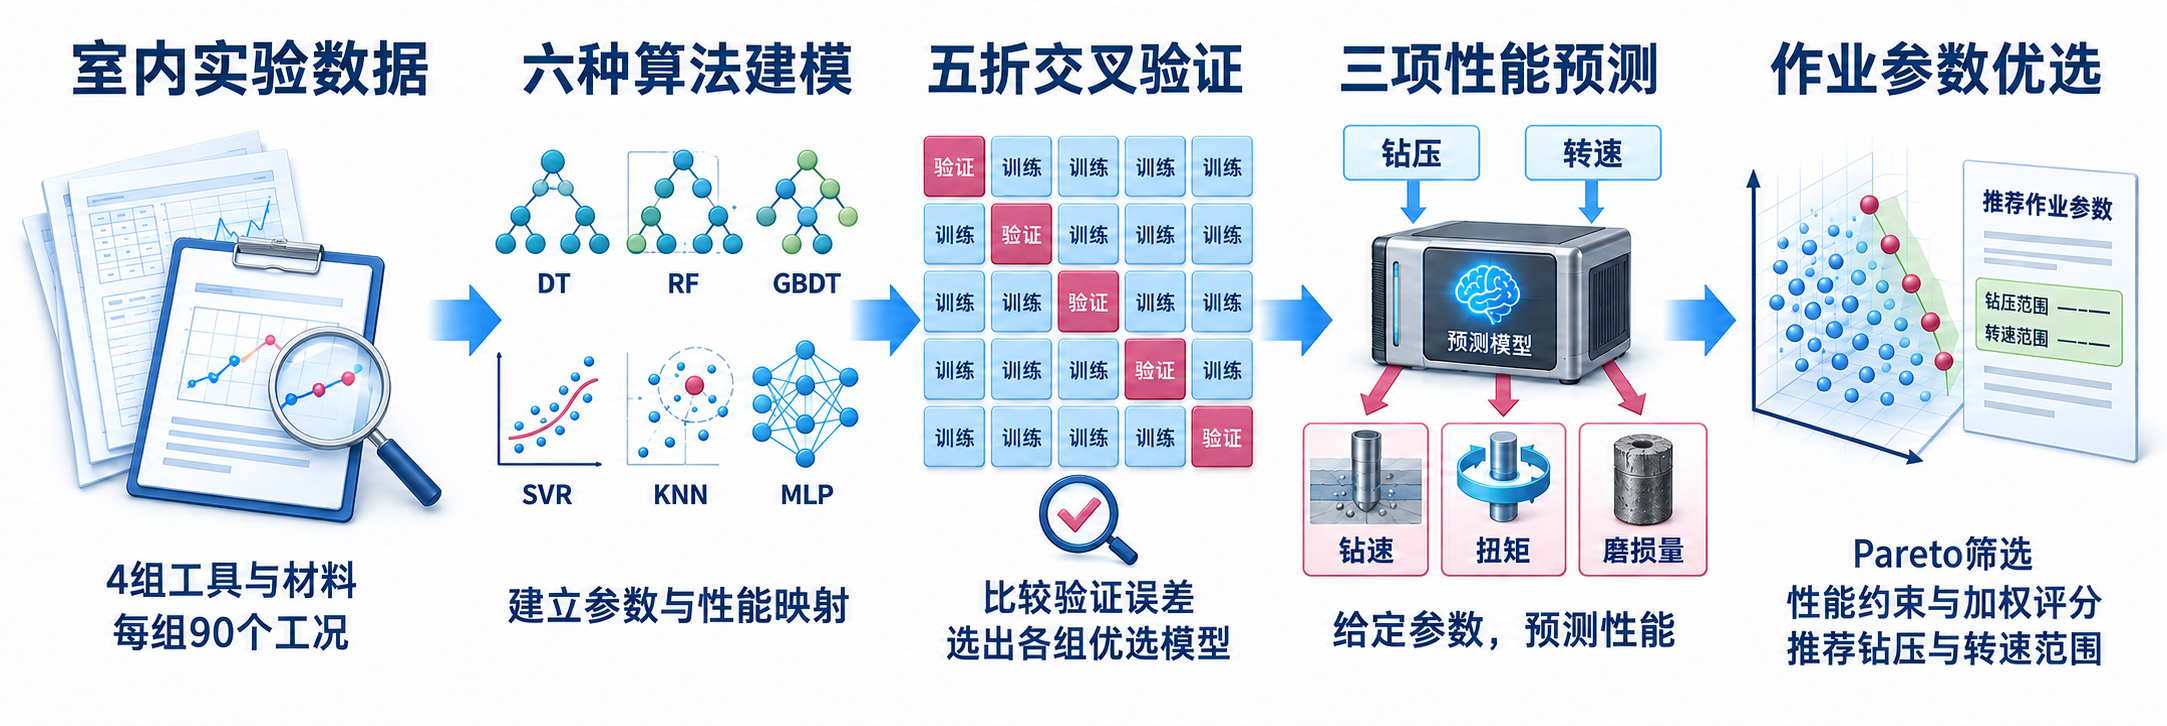
\includegraphics[width=145.000mm,height=0.76\textheight,keepaspectratio]{figure/research4-6/fig5-08-1.png}
\caption{室内实验数据建模与作业参数优化流程}
\label{fig:r46-5-8}
\end{figure}

\subsection{预测模型建立与选择}
\label{sec:r46-5.2.2}

采用多层感知机（MLP）、支持向量回归（SVR）、K近邻回归（KNN）、决策树（DT）、随机森林（RF）和梯度提升回归树（GBDT）建立性能预测模型。采用五折交叉验证，将各组数据分为五份，轮流用其中一份检验、其余四份训练，以未参与当次训练的数据计算预测误差。根据钻速、扭矩和磨损量的均方根误差（RMSE）比较模型表现，误差越小，预测值与实验值越接近。

四组数据选用的模型及交叉验证误差见表5-4。平底式磨铣采用随机森林，刀翼式磨铣采用多层感知机，套铣45号钢采用支持向量回归，套铣铸铁采用多层感知机。各组按自身实验数据选择模型，分别用于后续参数搜索。

\begin{table}[H]
\centering
\setstretch{1}
\fontsize{12}{15}\selectfont
\setlength{\tabcolsep}{3pt}
\renewcommand{\arraystretch}{1.5}
\caption{四组性能预测模型及交叉验证RMSE}\label{tab:r46-5-4}
\begin{tabular}{>{\centering\arraybackslash}m{0.286695\dimexpr\linewidth-10\tabcolsep-6\arrayrulewidth\relax}>{\centering\arraybackslash}m{0.095605\dimexpr\linewidth-10\tabcolsep-6\arrayrulewidth\relax}>{\centering\arraybackslash}m{0.211559\dimexpr\linewidth-10\tabcolsep-6\arrayrulewidth\relax}>{\centering\arraybackslash}m{0.204816\dimexpr\linewidth-10\tabcolsep-6\arrayrulewidth\relax}>{\centering\arraybackslash}m{0.201325\dimexpr\linewidth-10\tabcolsep-6\arrayrulewidth\relax}}
\toprule
 工具与材料 & 预测模型 & 钻速\newline{}(mm/min) & 扭矩\newline{}(N·m) & 磨损量\newline{}(g) \\ \midrule
平底式磨铣/45号钢 & RF & 0.494 & 2.387 & 0.190 \\ 
刀翼式磨铣/45号钢 & MLP & 0.574 & 2.583 & 0.155 \\ 
套铣/45号钢 & SVR & 0.809 & 4.531 & 0.465 \\ 
套铣/铸铁 & MLP & 0.789 & 5.928 & 0.708 \\ \bottomrule
\end{tabular}
\end{table}

\subsection{三项性能的预测结果}
\label{sec:r46-5.2.3}

四组模型的钻速RMSE为$0.494\sim0.809$ mm/min，扭矩RMSE为$2.387\sim5.928$ N·m，磨损量RMSE为$0.155\sim0.708$ g。钻速的决定系数R²为$0.935\sim0.964$，磨损量为$0.913\sim0.986$，扭矩为$0.644\sim0.819$。各工具与材料的模型及误差分别列于表5-4，作为相应组别参数搜索的依据。

图5-9至图5-11分别给出钻速、扭矩和磨损量的预测值与实验值对比，虚线表示两者相等。图中四组分别为平底式磨铣/45号钢、刀翼式磨铣/45号钢、套铣/45号钢和套铣/铸铁，与第四章实验分组一致。

\begin{figure}[H]
\centering
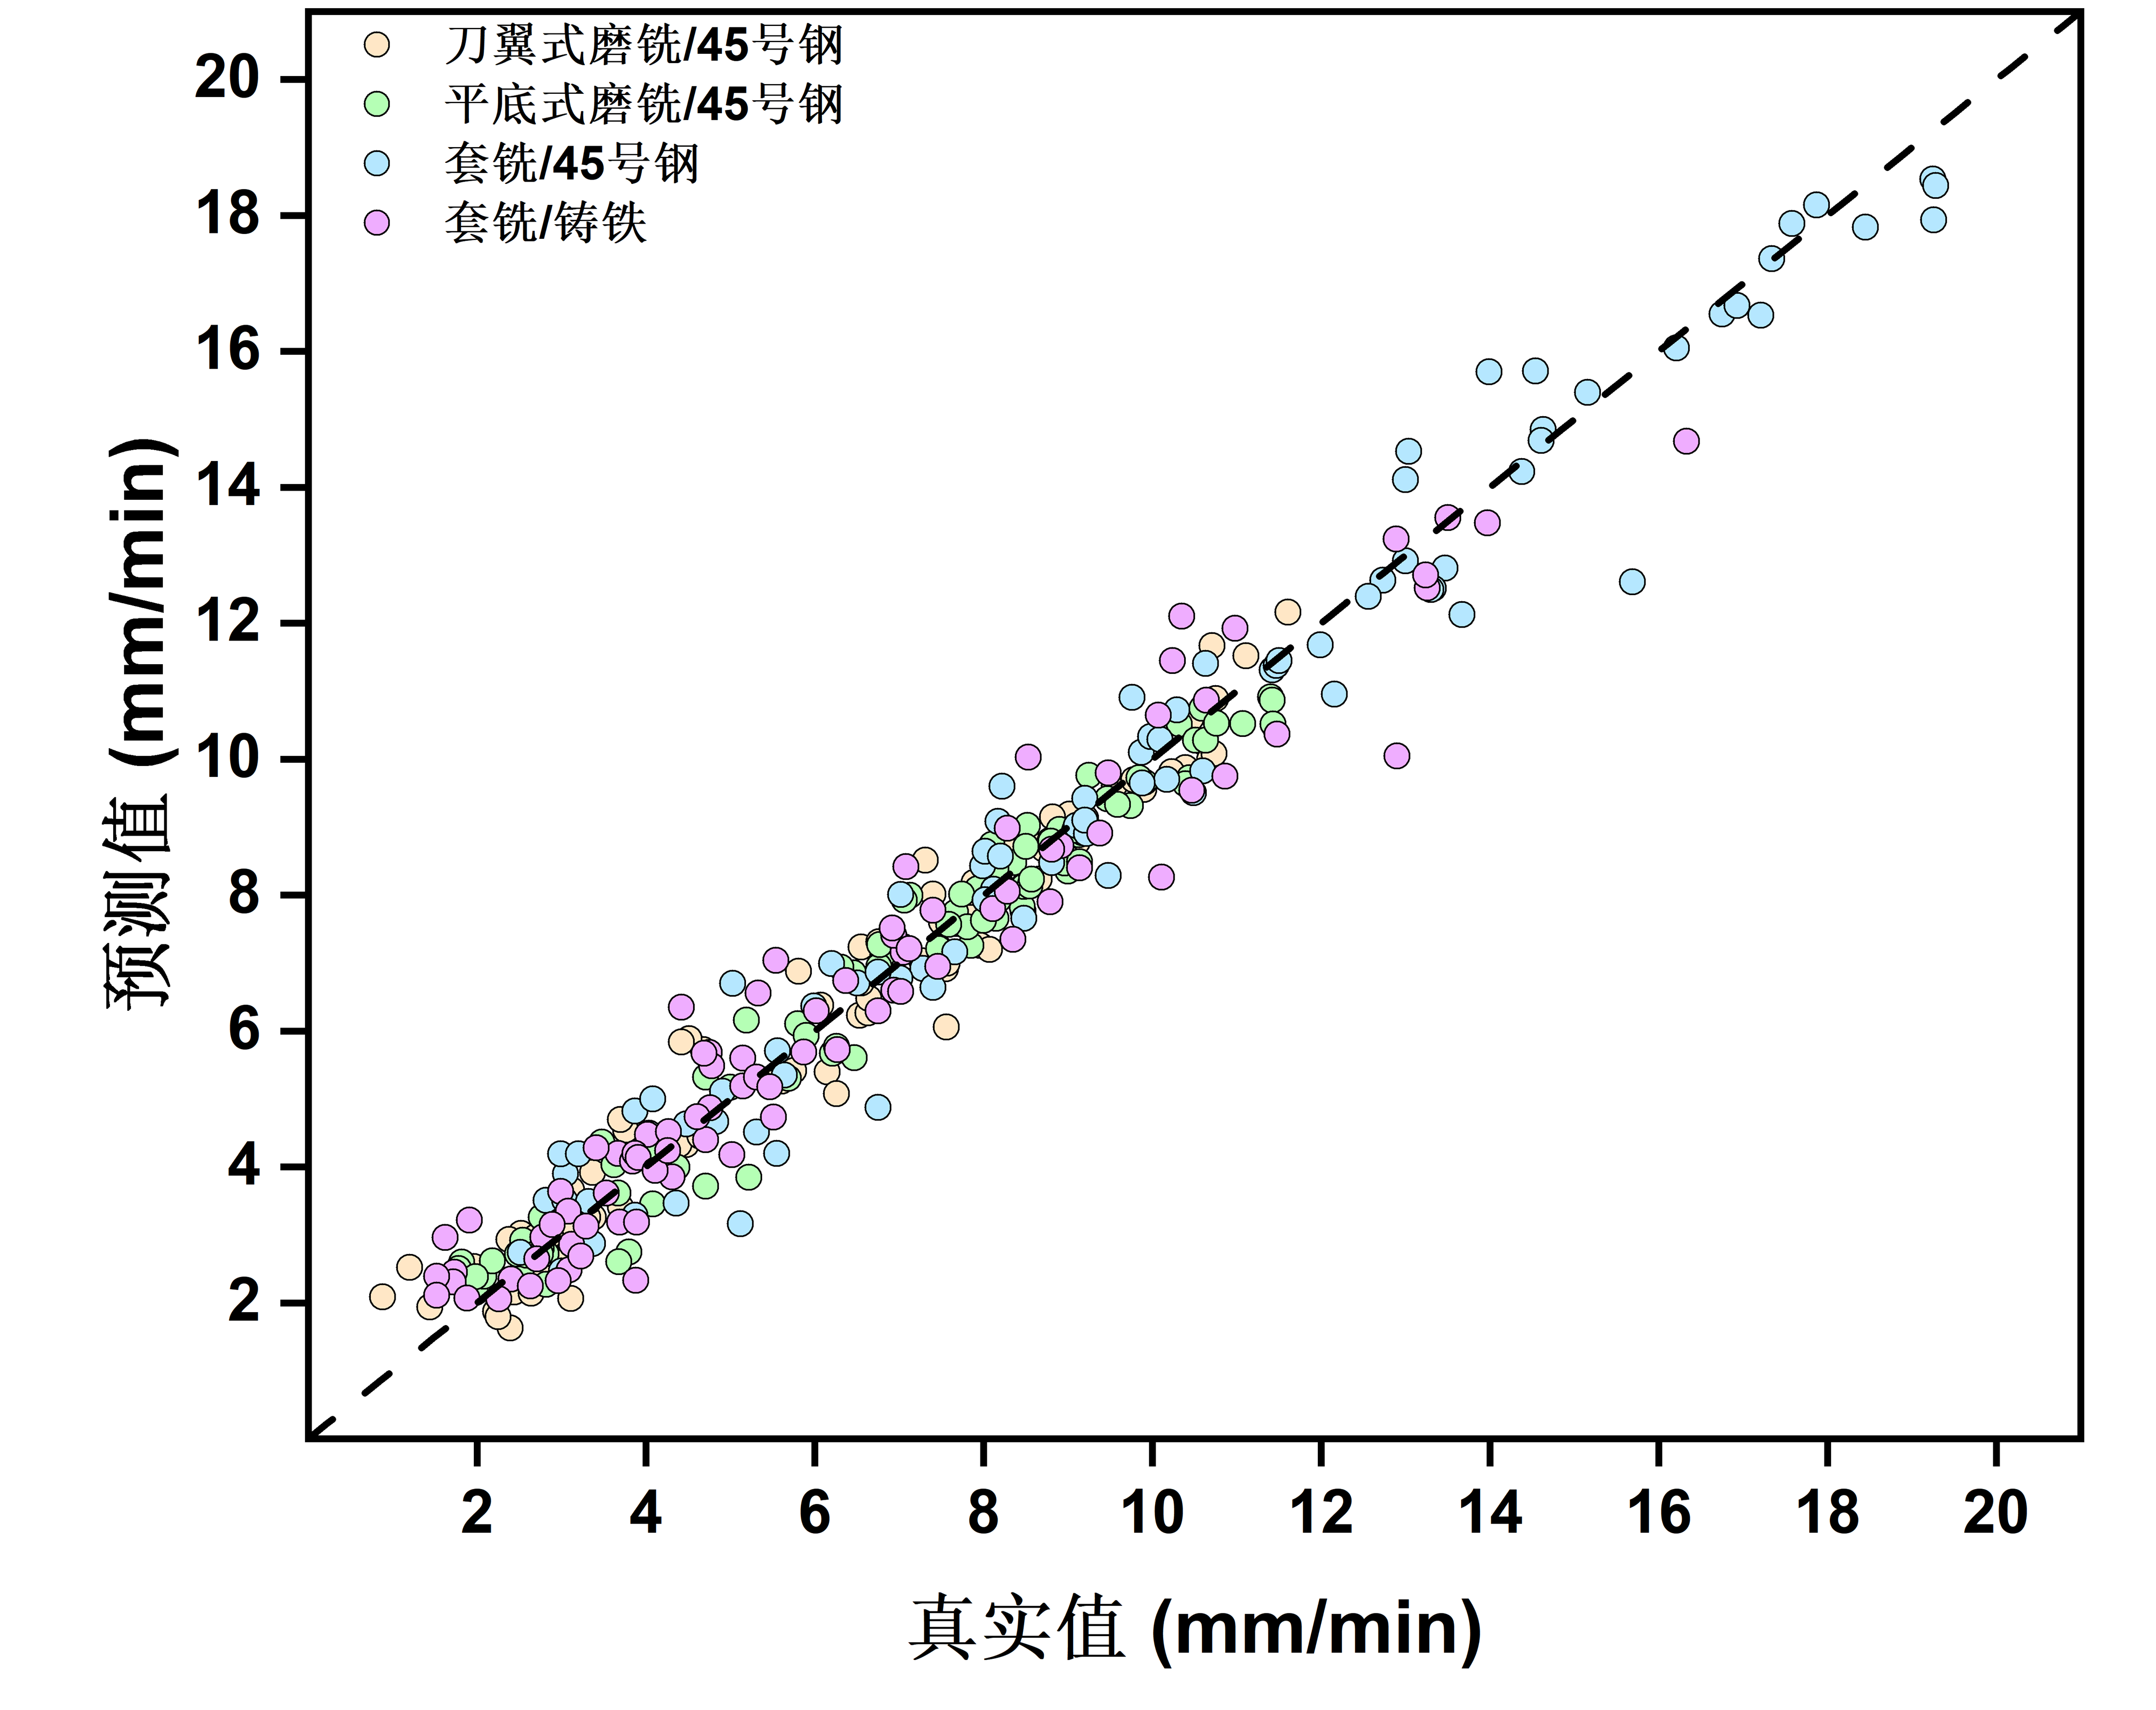
\includegraphics[width=136.000mm,height=0.76\textheight,keepaspectratio]{figure/research4-6/fig5-09-1.png}
\caption{四组工具钻速预测值与实验值对比}
\label{fig:r46-5-9}
\end{figure}

\begin{figure}[H]
\centering
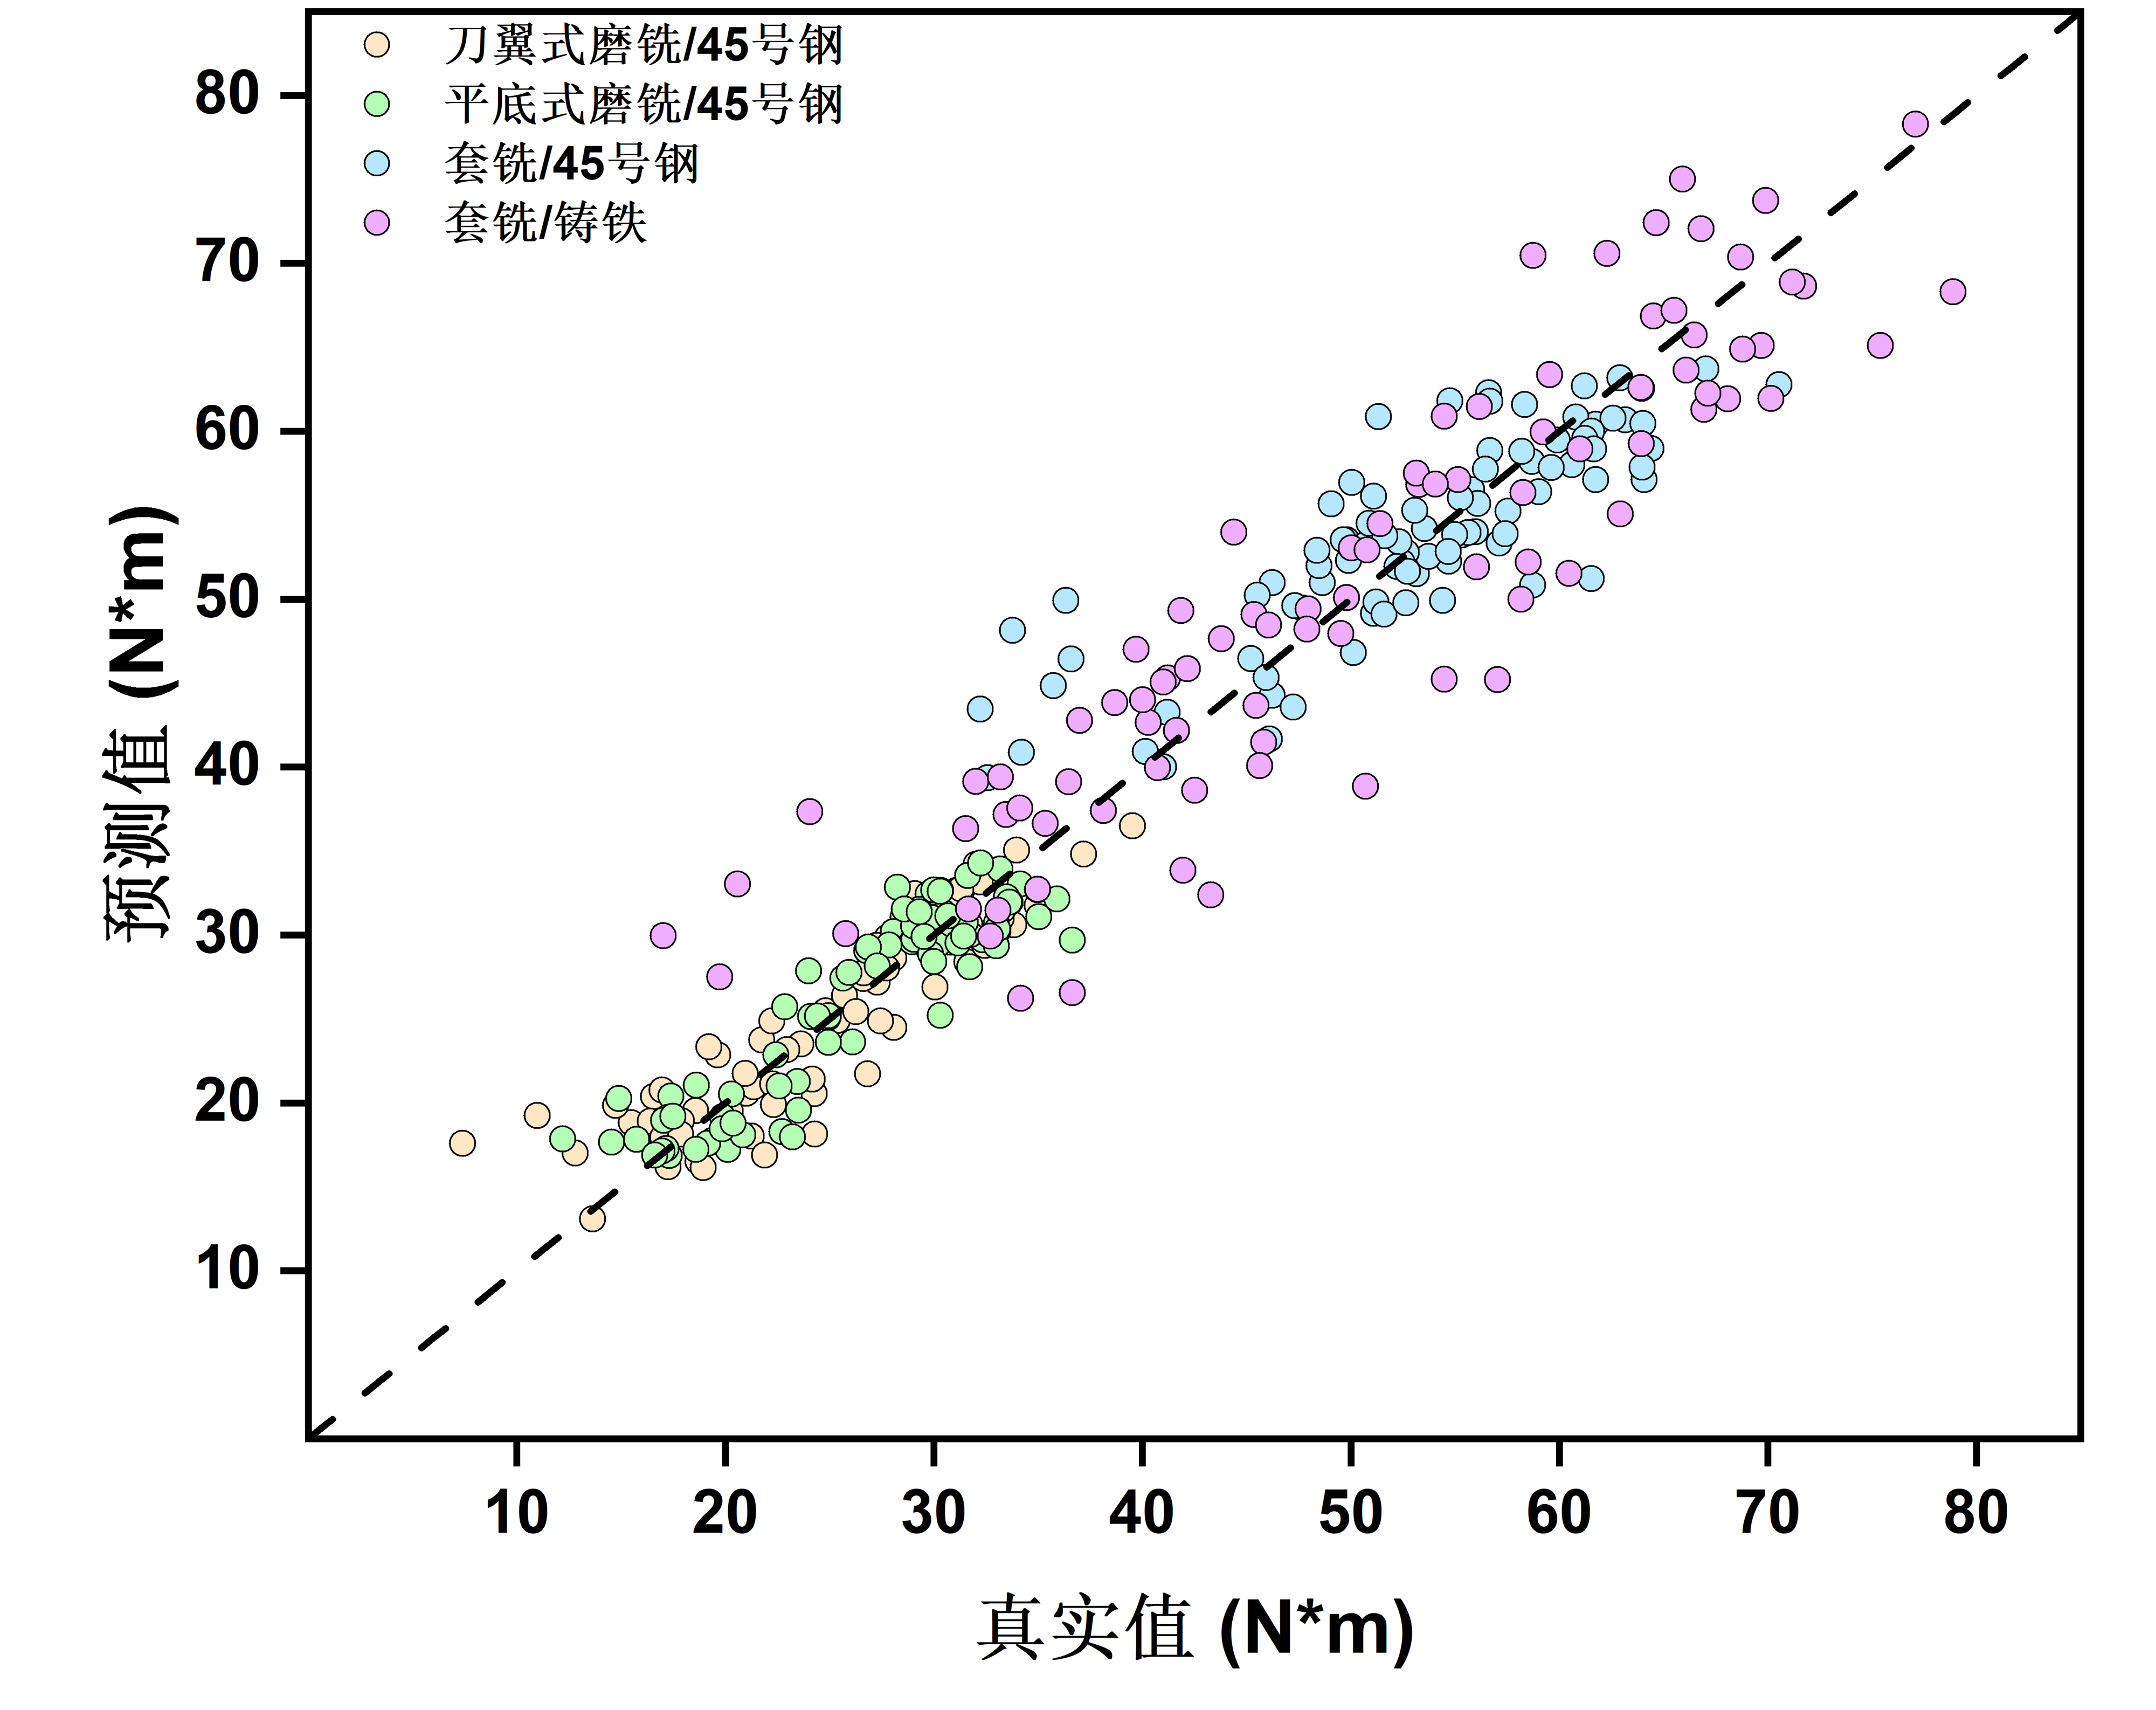
\includegraphics[width=136.000mm,height=0.76\textheight,keepaspectratio]{figure/research4-6/fig5-10-1.png}
\caption{四组工具扭矩预测值与实验值对比}
\label{fig:r46-5-10}
\end{figure}

\begin{figure}[H]
\centering
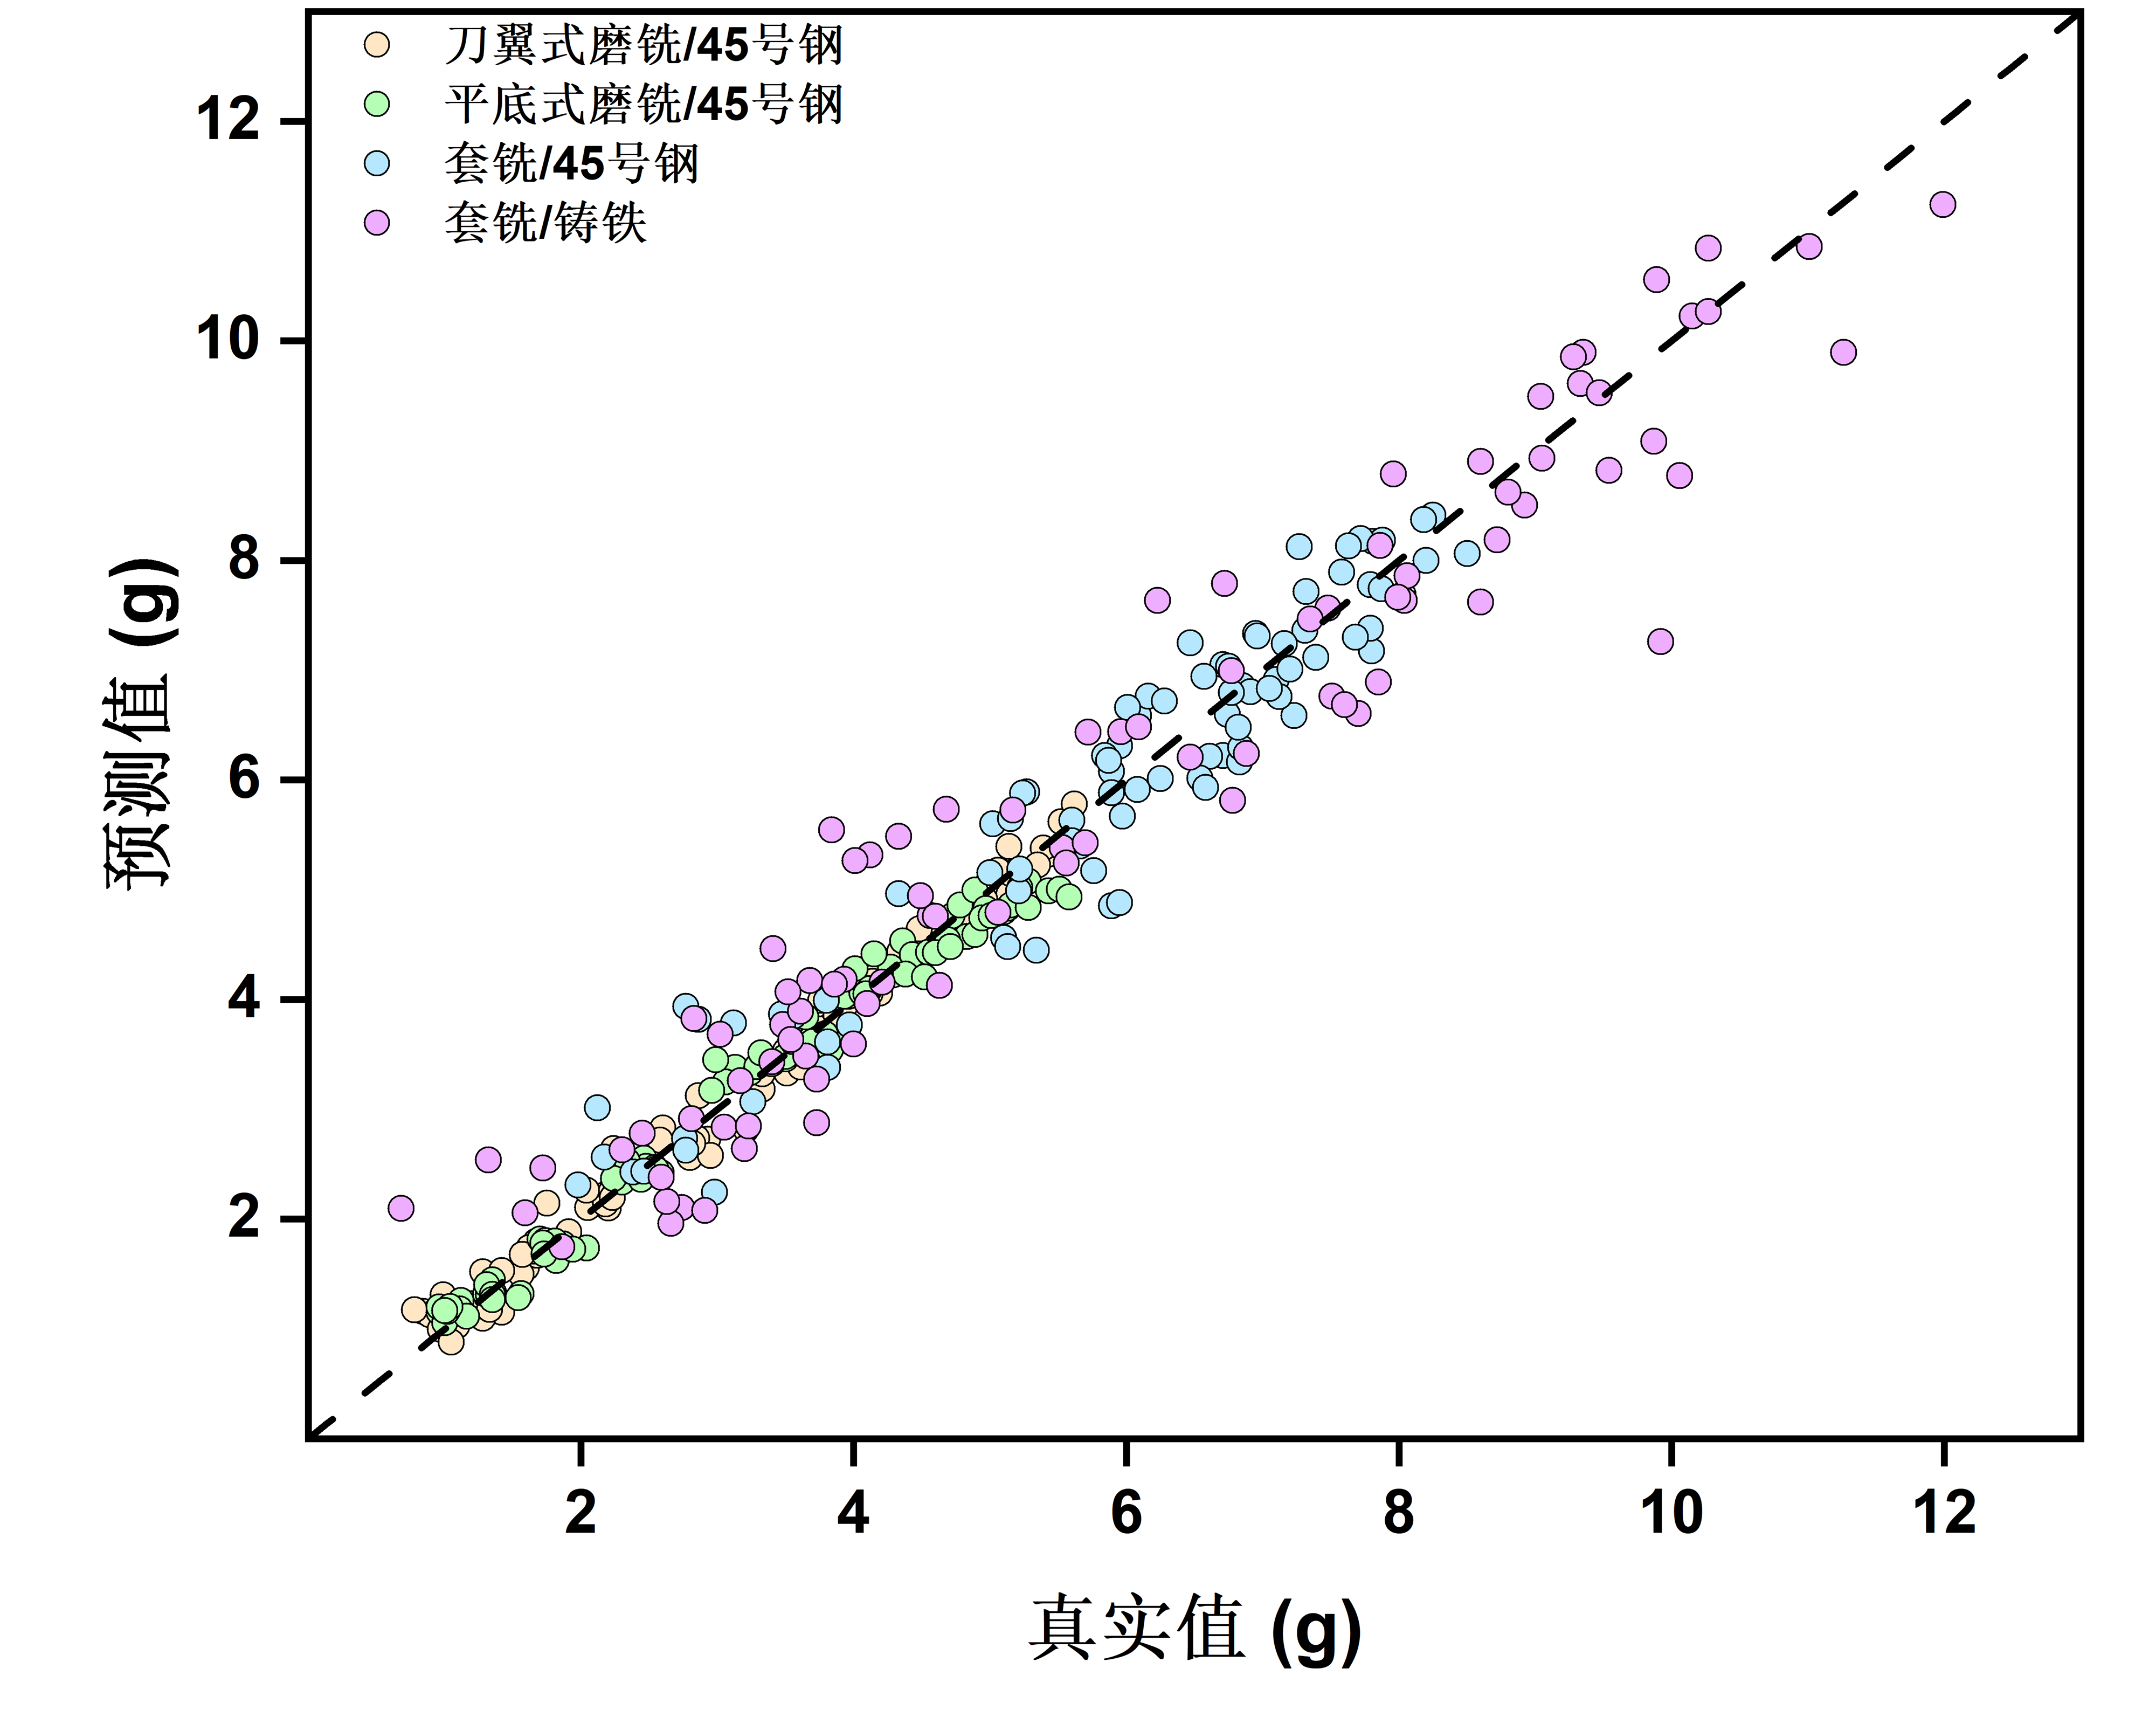
\includegraphics[width=136.000mm,height=0.76\textheight,keepaspectratio]{figure/research4-6/fig5-11-1.png}
\caption{四组工具磨损量预测值与实验值对比}
\label{fig:r46-5-11}
\end{figure}

\section{多目标作业参数优选}
\label{sec:r46-5.3}

\subsection{参数搜索与非支配筛选}
\label{sec:r46-5.3.1}

在实验覆盖的钻压$2\sim20$ kN、转速$20\sim100$ r/min范围内，每组计算6561种钻压与转速组合的预测性能，以提高钻速、降低扭矩和减少磨损量为优化目标，比较加工速度与负载、磨损之间的取舍。

采用Pareto非支配筛选比较候选组合。如果另一个组合的钻速不低、扭矩和磨损量均不高，且至少一项更好，则原组合不再保留。筛选后得到的非支配组合反映三项性能之间的取舍：继续提高其中一项性能，通常需要接受另一项性能的变化。四组分别得到4320、1924、967和242个非支配组合，结果见表5-5。

\subsection{性能要求与综合评分}
\label{sec:r46-5.3.2}

在非支配组合中，依据预测结果的分位数设定最低钻速、最大扭矩和最大磨损量，按“钻速保持在中高水平，优先控制扭矩并兼顾磨损量”的原则进一步筛选。表5-5列出本算例采用的筛选条件。

\begin{table}[H]
\centering
\setstretch{1}
\fontsize{12}{15}\selectfont
\setlength{\tabcolsep}{3pt}
\renewcommand{\arraystretch}{1.5}
\caption{非支配组合数量及算例筛选条件}\label{tab:r46-5-5}
\begin{tabular}{>{\centering\arraybackslash}m{0.300337\dimexpr\linewidth-10\tabcolsep-6\arrayrulewidth\relax}>{\centering\arraybackslash}m{0.122832\dimexpr\linewidth-10\tabcolsep-6\arrayrulewidth\relax}>{\centering\arraybackslash}m{0.191113\dimexpr\linewidth-10\tabcolsep-6\arrayrulewidth\relax}>{\centering\arraybackslash}m{0.191113\dimexpr\linewidth-10\tabcolsep-6\arrayrulewidth\relax}>{\centering\arraybackslash}m{0.194605\dimexpr\linewidth-10\tabcolsep-6\arrayrulewidth\relax}}
\toprule
 工具与材料 & 非支配\newline{}组合数 & 最低钻速\newline{}(mm/min) & 最大扭矩\newline{}(N·m) & 最大磨损量\newline{}(g) \\ \midrule
平底式磨铣/45号钢 & 4320 & 6.5258 & 29.5389 & 4.1161 \\ 
刀翼式磨铣/45号钢 & 1924 & 5.9566 & 30.0575 & 4.8497 \\ 
套铣/45号钢 & 967 & 11.5061 & 52.8552 & 6.8853 \\ 
套铣/铸铁 & 242 & 12.4356 & 70.0142 & 10.7606 \\ \bottomrule
\end{tabular}
\end{table}

对满足条件的组合，将三项性能归一化后进行加权评分，按钻速提高、扭矩降低和磨损减少的方向比较，再按综合得分排序，输出钻压、转速及对应的三项预测性能。

\section{不同工具和材料的参数优化结果}
\label{sec:r46-5.4}

\subsection{推荐参数及预测性能}
\label{sec:r46-5.4.1}

四组推荐结果的预测性能范围见表5-6。平底式磨铣在钻速约$7.37\sim7.40$ mm/min时，将预测扭矩控制在约$27.54\sim27.67$ N·m；刀翼式磨铣推荐区域的预测钻速约$5.96\sim6.35$ mm/min，同时对应较低的扭矩和磨损量。套铣两种材料的推荐区域不同，应分别采用相应模型和筛选条件。

\begin{table}[H]
\centering
\setstretch{1}
\fontsize{12}{15}\selectfont
\setlength{\tabcolsep}{3pt}
\renewcommand{\arraystretch}{1.5}
\caption{推荐组合的预测性能范围}\label{tab:r46-5-6}
\begin{tabular}{>{\centering\arraybackslash}m{0.286695\dimexpr\linewidth-8\tabcolsep-5\arrayrulewidth\relax}>{\centering\arraybackslash}m{0.238892\dimexpr\linewidth-8\tabcolsep-5\arrayrulewidth\relax}>{\centering\arraybackslash}m{0.238892\dimexpr\linewidth-8\tabcolsep-5\arrayrulewidth\relax}>{\centering\arraybackslash}m{0.235521\dimexpr\linewidth-8\tabcolsep-5\arrayrulewidth\relax}}
\toprule
 工具与材料 & 预测钻速\newline{}(mm/min) & 预测扭矩\newline{}(N·m) & 预测磨损量\newline{}(g) \\ \midrule
平底式磨铣/45号钢 & $7.3707\sim7.3980$ & $27.5443\sim27.6652$ & $4.0791\sim4.1092$ \\ 
刀翼式磨铣/45号钢 & $5.9593\sim6.3451$ & $24.4922\sim25.3742$ & $2.6586\sim2.9897$ \\ 
套铣/45号钢 & $11.5075\sim12.6766$ & $51.7816\sim52.0882$ & $6.7320\sim6.8850$ \\ 
套铣/铸铁 & $12.4419\sim13.7041$ & $64.8384\sim69.9896$ & $9.4340\sim10.6947$ \\ \bottomrule
\end{tabular}
\end{table}

\begin{table}[H]
\centering
\setstretch{1}
\fontsize{12}{15}\selectfont
\setlength{\tabcolsep}{3pt}
\renewcommand{\arraystretch}{1.5}
\caption{各组推荐参数及其预测性能示例}\label{tab:r46-5-7}
\begin{tabular}{>{\centering\arraybackslash}m{0.259393\dimexpr\linewidth-12\tabcolsep-7\arrayrulewidth\relax}>{\centering\arraybackslash}m{0.095617\dimexpr\linewidth-12\tabcolsep-7\arrayrulewidth\relax}>{\centering\arraybackslash}m{0.102360\dimexpr\linewidth-12\tabcolsep-7\arrayrulewidth\relax}>{\centering\arraybackslash}m{0.180877\dimexpr\linewidth-12\tabcolsep-7\arrayrulewidth\relax}>{\centering\arraybackslash}m{0.180877\dimexpr\linewidth-12\tabcolsep-7\arrayrulewidth\relax}>{\centering\arraybackslash}m{0.180877\dimexpr\linewidth-12\tabcolsep-7\arrayrulewidth\relax}}
\toprule
 工具与材料 & 钻压\newline{}(kN) & 转速\newline{}(r/min) & 预测钻速\newline{}(mm/min) & 预测扭矩\newline{}(N·m) & 预测磨损量\newline{}(g) \\ \midrule
平底式磨铣/45号钢 & 16.625 & 22 & 7.3980 & 27.5443 & 4.1092 \\ 
刀翼式磨铣/45号钢 & 8.750 & 100 & 5.9593 & 24.7121 & 2.6586 \\ 
套铣/45号钢 & 18.650 & 50 & 11.5075 & 51.7816 & 6.7381 \\ 
套铣/铸铁 & 15.725 & 100 & 12.5579 & 64.8384 & 9.4433 \\ \bottomrule
\end{tabular}
\end{table}

\subsection{三项性能的权衡关系}
\label{sec:r46-5.4.2}

图5-12至图5-15以预测钻速为横坐标、预测扭矩为纵坐标，并用颜色表示预测磨损量。红色点及圈定区域表示经性能约束和综合评分得到的推荐工况。四图依次对应平底式磨铣加工45号钢、刀翼式磨铣加工45号钢、套铣加工45号钢和套铣加工铸铁，与表5-5至表5-7的分组相同。

\begin{figure}[H]
\centering
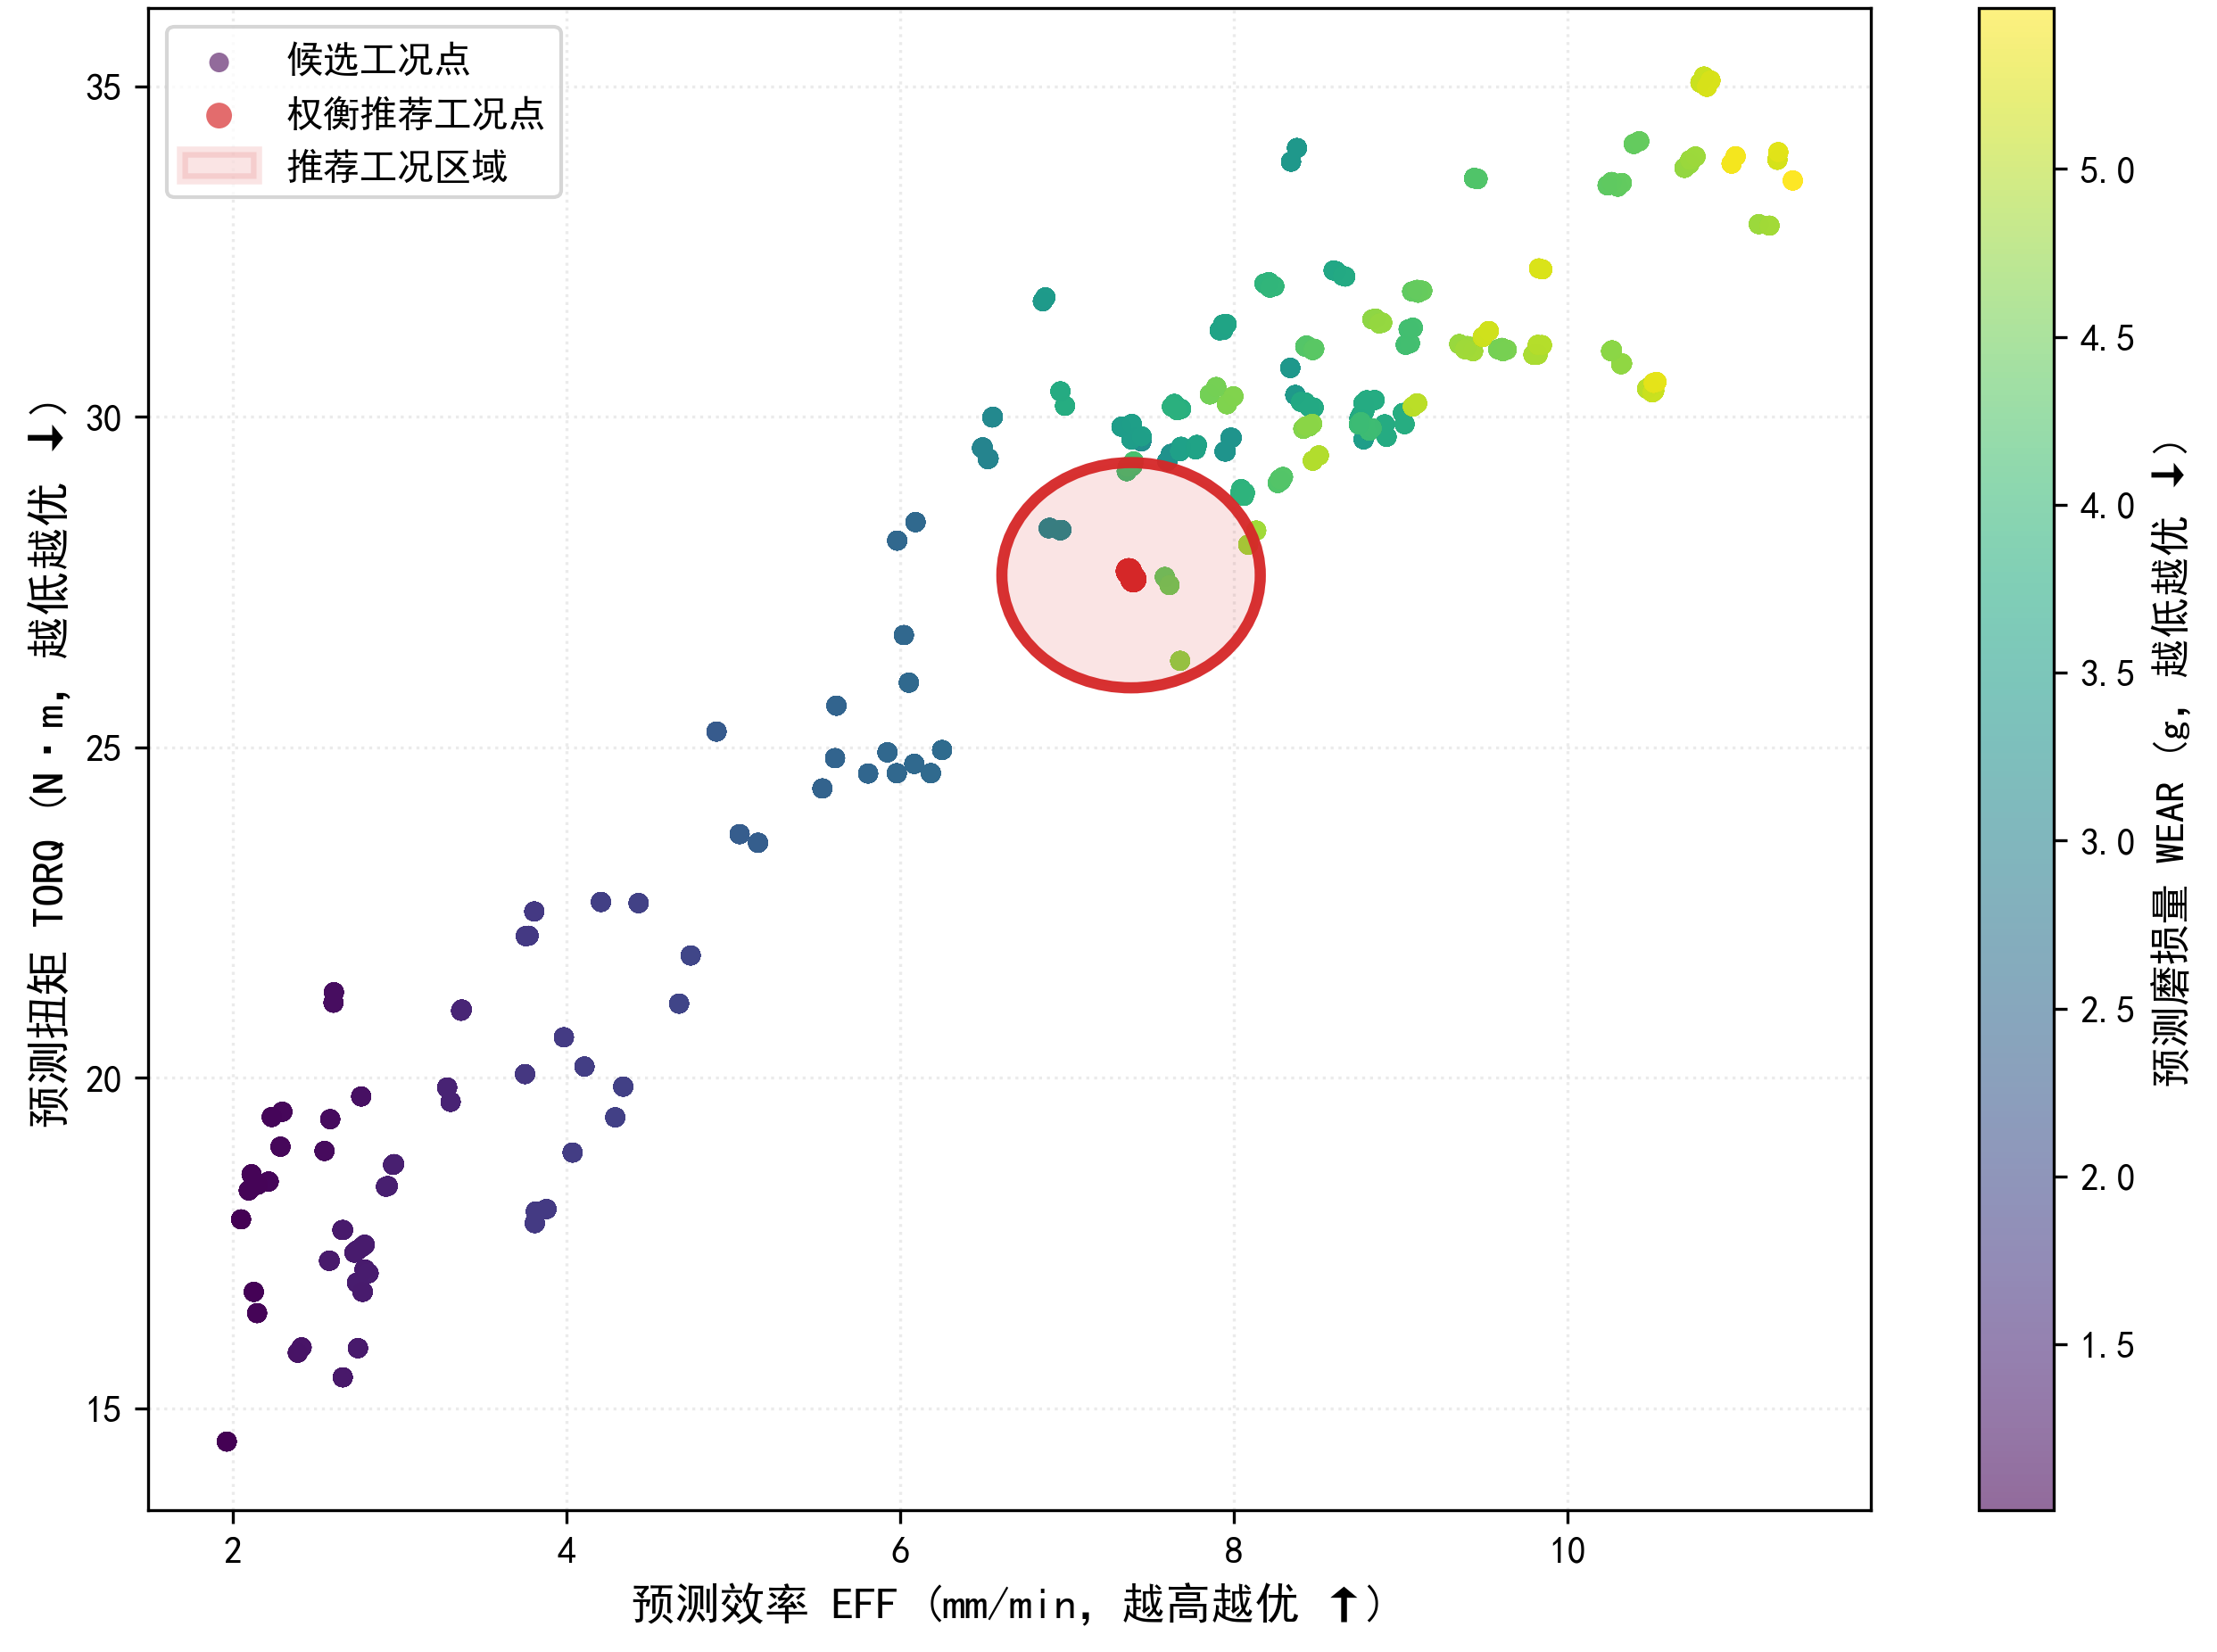
\includegraphics[width=145.000mm,height=0.76\textheight,keepaspectratio]{figure/research4-6/fig5-12-1.png}
\caption{平底式磨铣加工45号钢的性能权衡及推荐区域}
\label{fig:r46-5-12}
\end{figure}

\begin{figure}[H]
\centering
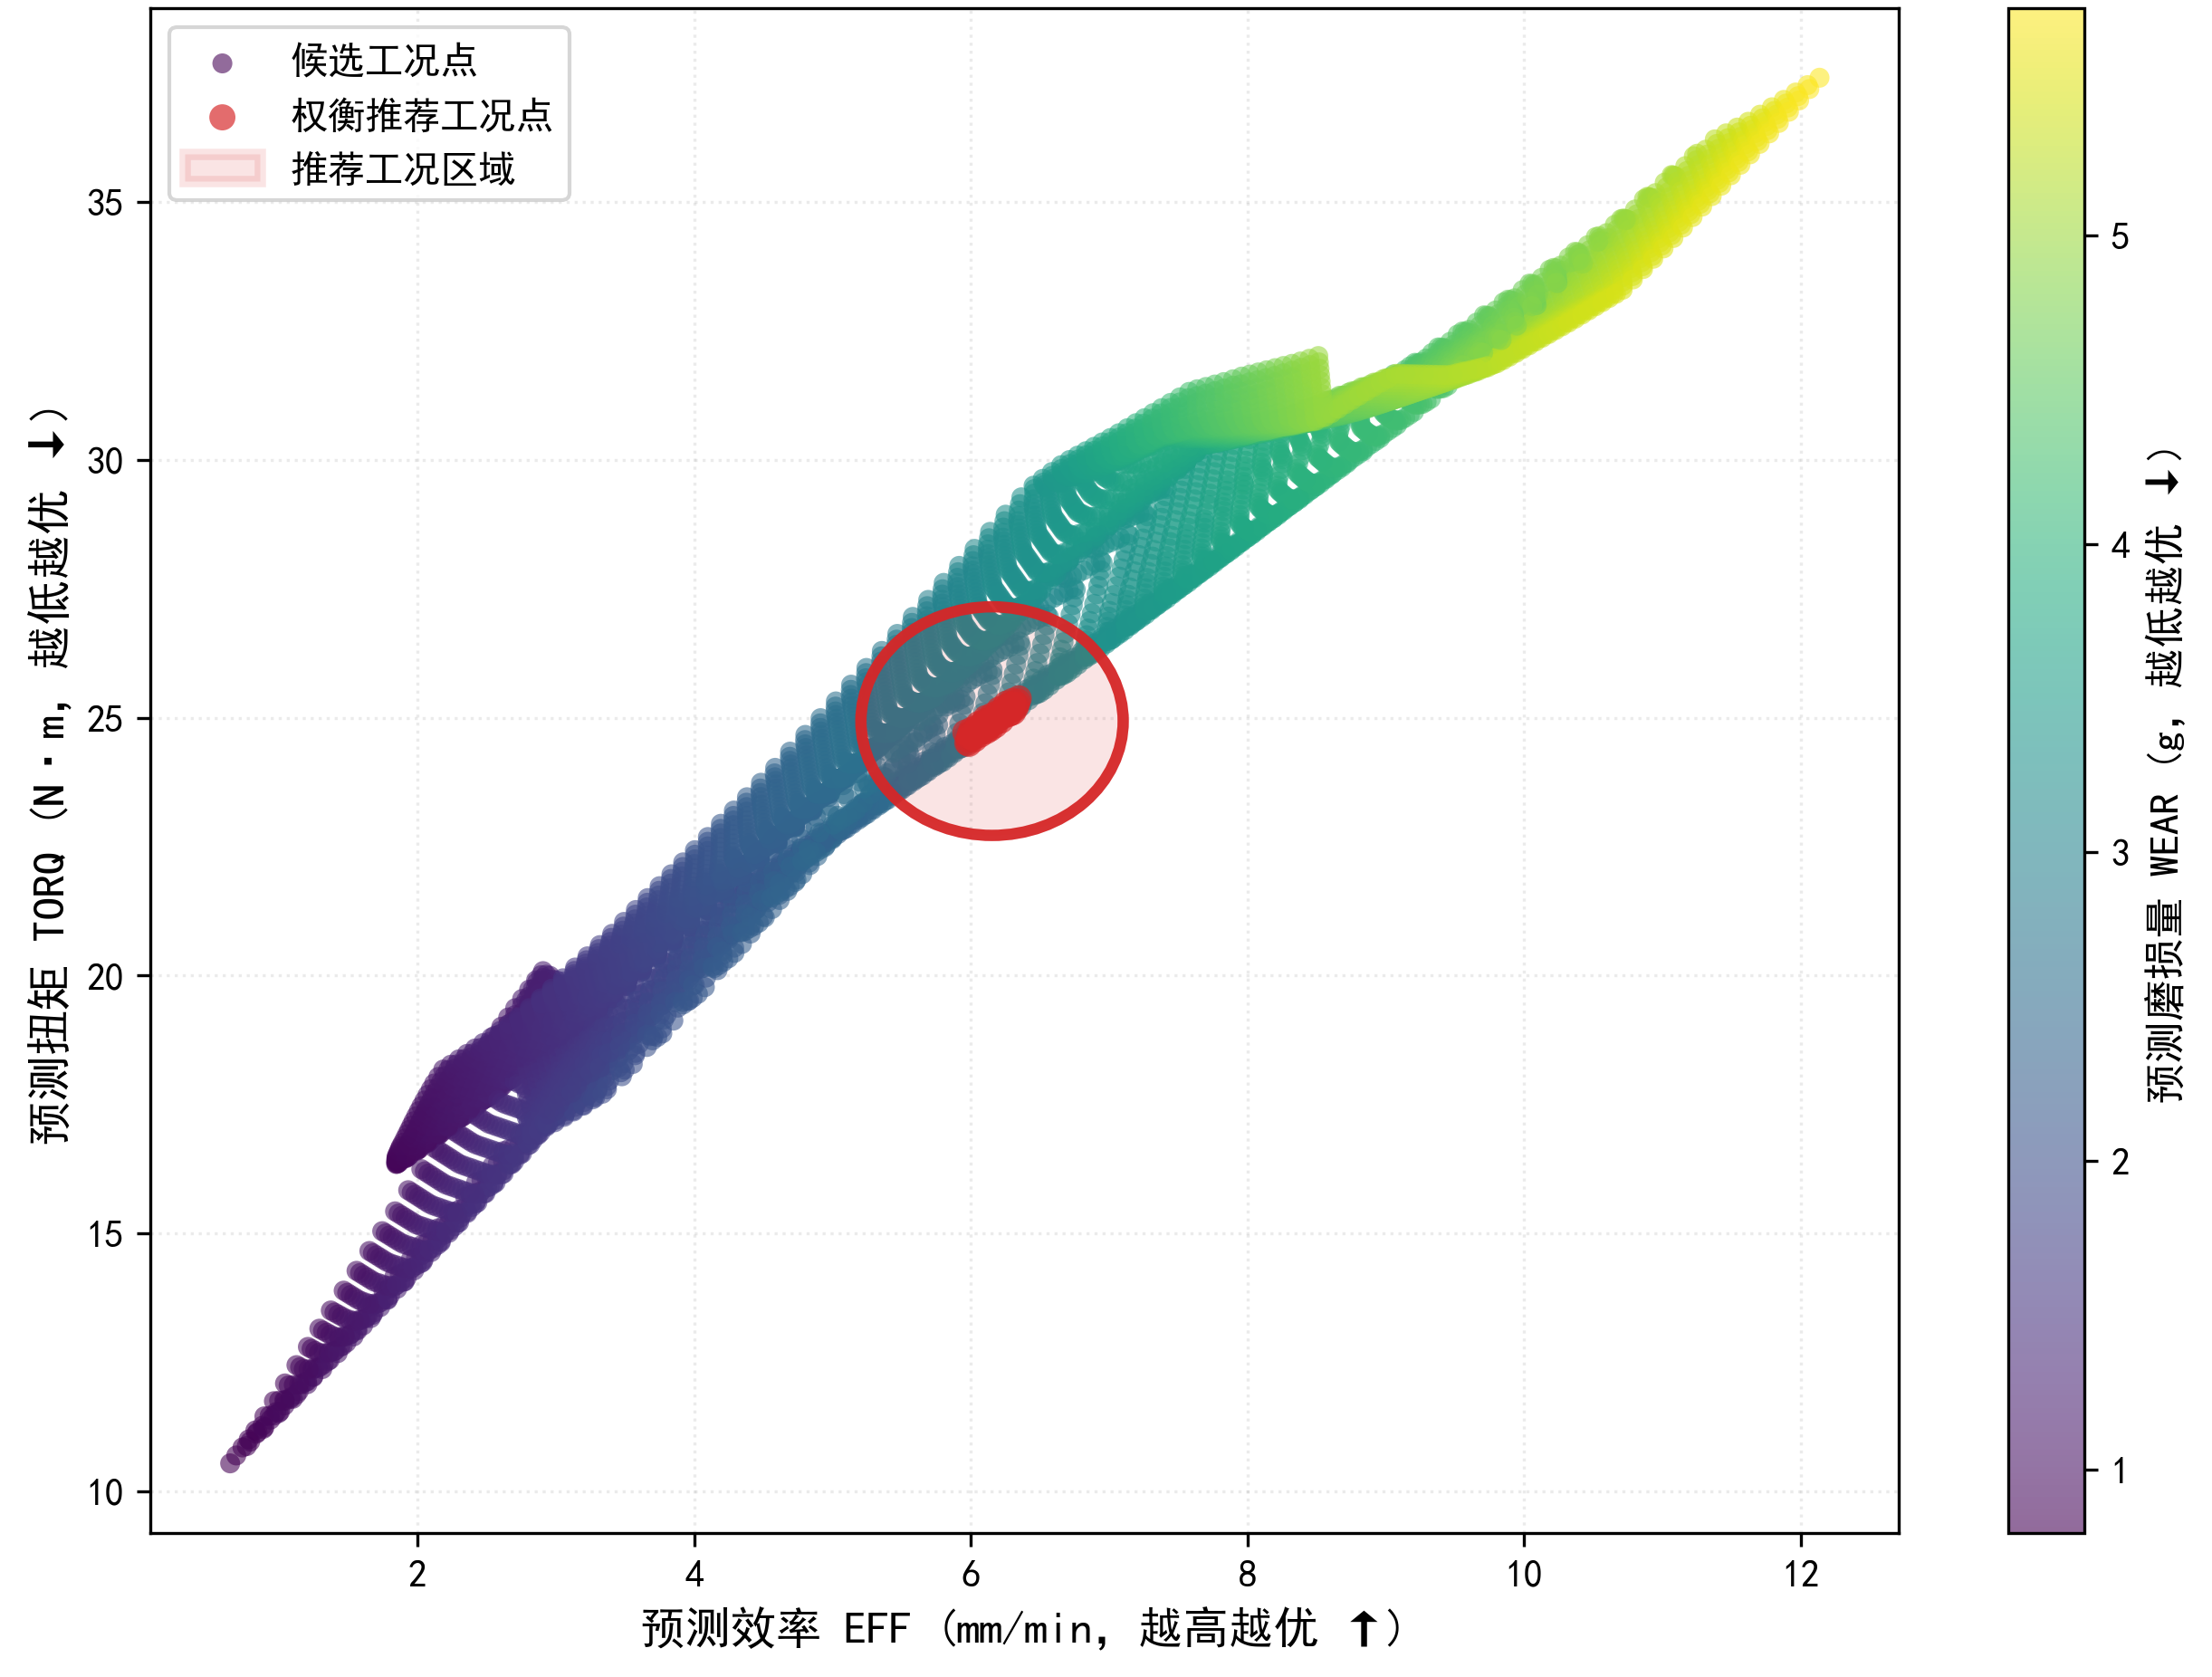
\includegraphics[width=145.000mm,height=0.76\textheight,keepaspectratio]{figure/research4-6/fig5-13-1.png}
\caption{刀翼式磨铣加工45号钢的性能权衡及推荐区域}
\label{fig:r46-5-13}
\end{figure}

套铣45号钢的推荐点位于较低扭矩对应的性能分布下缘，在保持钻速要求的同时控制负载；套铣铸铁的推荐点集中在较高钻速区域，扭矩和磨损量也相应较高。两组结果体现了材料变化后的性能差异及推荐范围。

\begin{figure}[H]
\centering
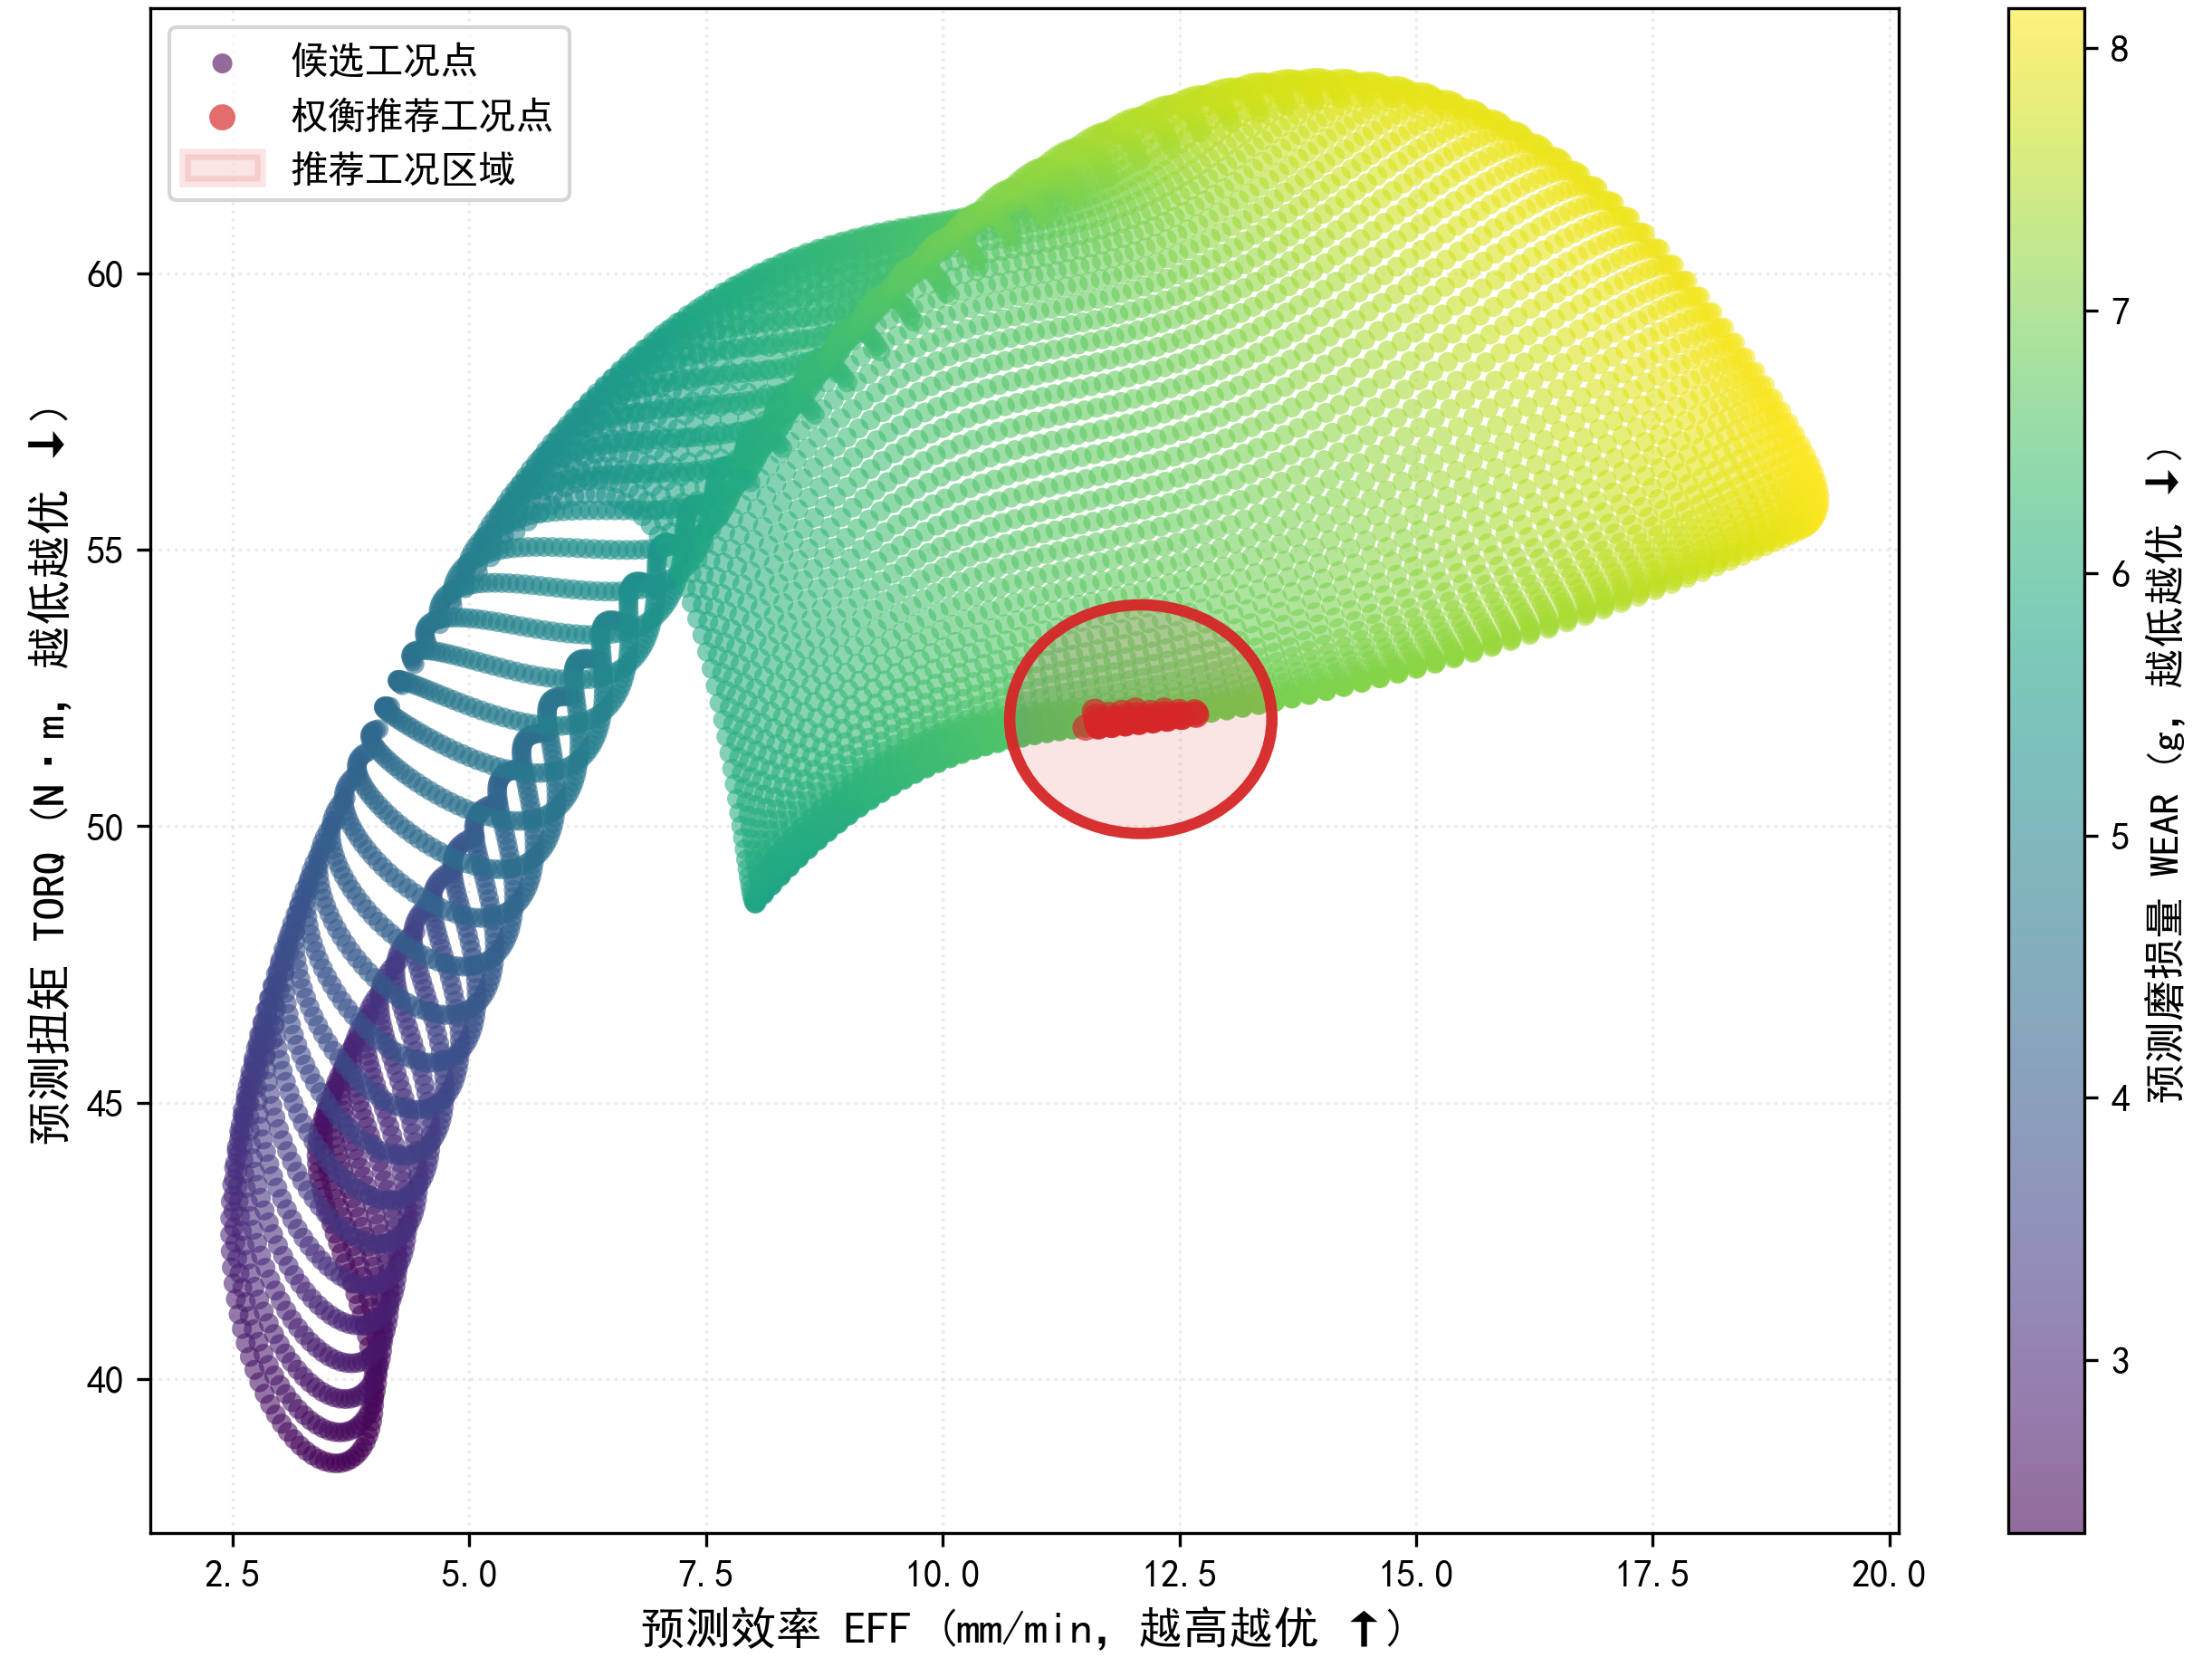
\includegraphics[width=145.000mm,height=0.76\textheight,keepaspectratio]{figure/research4-6/fig5-14-1.png}
\caption{套铣加工45号钢的性能权衡及推荐区域}
\label{fig:r46-5-14}
\end{figure}

\begin{figure}[H]
\centering
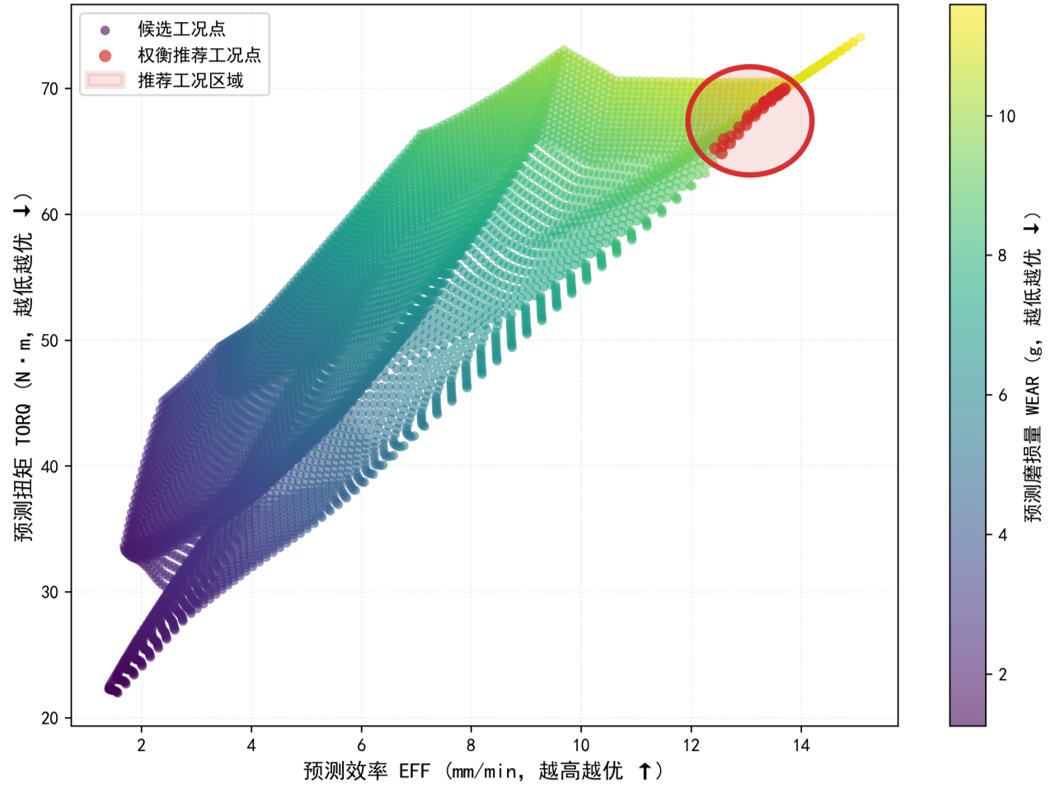
\includegraphics[width=145.000mm,height=0.76\textheight,keepaspectratio]{figure/research4-6/fig5-15-1.png}
\caption{套铣加工铸铁的性能权衡及推荐区域}
\label{fig:r46-5-15}
\end{figure}

\section{正向预测与目标参数反向推荐}
\label{sec:r46-5.5}

\subsection{两种参数计算方式}
\label{sec:r46-5.5.1}

正向预测由用户选择工具及工件材料，输入钻压和转速，计算钻速、扭矩及磨损量。反向推荐由用户输入目标性能，在实验范围内通过正向模型搜索候选组合，再按目标偏差和综合评分返回钻压、转速。两种计算方式共用相应工具与材料的正向预测模型。

平底式磨铣的交互算例见表5-8。正向计算输入15 kN钻压、50 r/min转速，得到预测钻速8.2166 mm/min、扭矩31.9562 N·m和磨损量3.9489 g。反向计算输入目标钻速8 mm/min、扭矩25 N·m和磨损量3 g，程序返回7.2800 kN和54.6667 r/min的参数组合，作为按该目标搜索得到的推荐设置。

\begin{table}[H]
\centering
\setstretch{1}
\fontsize{12}{15}\selectfont
\setlength{\tabcolsep}{3pt}
\renewcommand{\arraystretch}{1.5}
\caption{平底式磨铣正向预测与反向推荐算例}\label{tab:r46-5-8}
\begin{tabular}{>{\centering\arraybackslash}m{0.136528\dimexpr\linewidth-6\tabcolsep-4\arrayrulewidth\relax}>{\centering\arraybackslash}m{0.385625\dimexpr\linewidth-6\tabcolsep-4\arrayrulewidth\relax}>{\centering\arraybackslash}m{0.477847\dimexpr\linewidth-6\tabcolsep-4\arrayrulewidth\relax}}
\toprule
 计算方式 & 输入内容 & 输出结果 \\ \midrule
正向预测 & 钻压15 kN\newline{}转速50 r/min & 预测钻速8.2166 mm/min\newline{}预测扭矩31.9562 N·m\newline{}预测磨损量3.9489 g \\ 
反向推荐 & 目标钻速8 mm/min\newline{}目标扭矩25 N·m\newline{}目标磨损量3 g & 推荐钻压7.2800 kN\newline{}推荐转速54.6667 r/min \\ \bottomrule
\end{tabular}
\end{table}

\subsection{作业参数智能推荐系统}
\label{sec:r46-5.5.2}

套磨铣工具作业参数智能推荐系统集成工具与材料选择、性能预测和参数推荐功能。相关性分析、模型评价和Pareto优化视图分别显示数据关系、预测表现及候选工况的性能分布。图5-16给出套铣加工45号钢的相关性分析界面，其中钻压、转速与三项性能的关系对应第四章同组实验结果。

\begin{figure}[H]
\centering
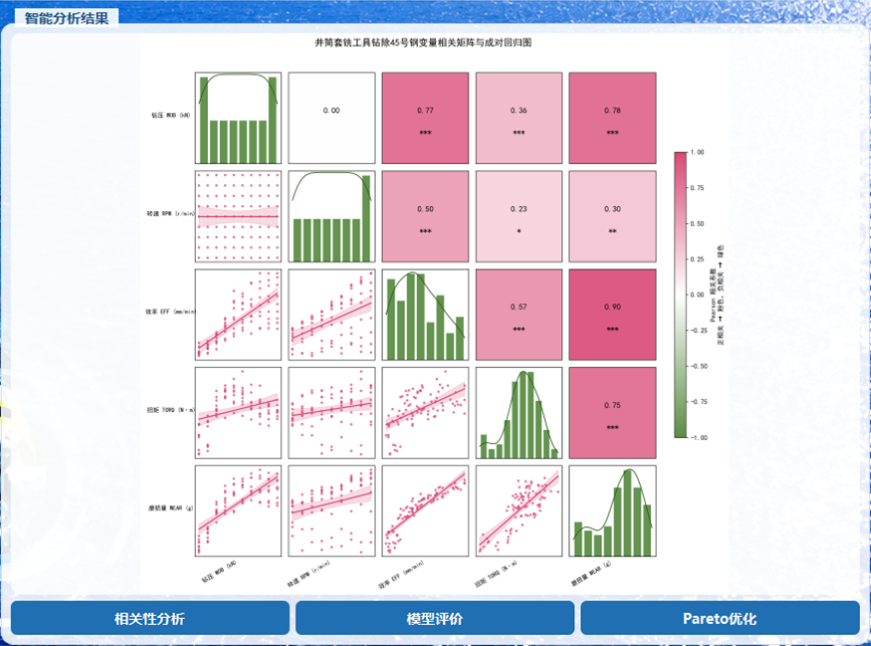
\includegraphics[width=132.000mm,height=0.76\textheight,keepaspectratio]{figure/research4-6/fig5-16-1.png}
\caption{套铣加工45号钢的相关性分析界面}
\label{fig:r46-5-16}
\end{figure}

使用时先选择工具类型与工件材料，再输入作业参数或目标性能，调用相应预测模型进行计算。平底式磨铣、刀翼式磨铣及套铣两种材料分别使用各自模型，按对应组别的性能分布和筛选条件推荐参数。
